\section{Results}\label{results}
This chapter presents the results of calibrating Model 1-4 with the MCMC samplers: AI, DE and DE-SNK, for the scenarios described above. The efficiency of the samplers is evaluated using acceptance rates and the estimated Effective Sample Size ($\widehat{ESS}$). Subsequently, chain convergence is assessed with the Gelman-Rubin diagnostic ($\hat{R}$). 
Next, samplers are compared based on how closely their posterior medians approximate the true hydraulic conductivities. 
Finally, the shape of the posterior distributions and the relationship between different parameters is investigated with Kernel Density Estimate plots (KDE) and pairs plots, respectively.   

The acceptance rate of proposed steps varies strongly between the different samplers, with the Affine-Invariant sampler (AI) reporting the highest acceptance rates (\hyperref[tab_fracs]{\textcolor{blue}{Table }\ref{tab_fracs}}). The observed acceptance rate for all samplers decreases when the number of calibrated parameters increases, considering that dimensionalities for Model 1 up to Model 4 are 1,2,3 and 5, respectively. 
The optimal acceptance rate according to theory is 0.44 for 1 dimension, decreasing to 0.28 for 5 dimensions and asymptotically approaching 0.23 for even higher dimensions \citep{schmon2022optimal, terbraak2006markov}. For DE-based strategies, most acceptance rates closely align with these optimal values. Except for too low values when using the wide prior for Model 3 and 4. In contrast, AI reports too high acceptance rates for most scenarios. Regarding prior choice, using the narrow prior resulted on average in more optimal acceptance rates for DE and DE-SNK, but not for AI. % caused by initialisation far true posterior density? OR due to prior shifted away from true posterior density? 
The variability in acceptance rates between chains of a specific sampler for a specific scenario is relatively small, indicated by the compactness of the boxplots, suggesting consistency between different ensembles (\hyperref[tab_fracs]{\textcolor{blue}{Table }\ref{tab_fracs}}).

\begin{table*}[ht]
\centering
\caption{Acceptance rates for each scenario are presented with boxplots. Each boxplot was constructed using acceptance rates of the last 1000 steps of 50 chains (5 ensembles of 10 chains). Optimal Metropolis acceptance rates, based on dimensionality, are indicated with dashed red lines: 0.44 for Model 1, 0.35 for Model 2, 0.31 for Model 3 and 0.28 for Model 4 \citep{schmon2022optimal}. Although invisible, all boxplots in the same column share the same x-axis and thus can be compared. Additionally, average row acceptance rates are provided in the rightmost column and average column acceptance rates are provided in the bottom row.}
\label{tab_fracs}
\begin{tabularx}{\textwidth}{llXXXXXXl}
\toprule
\multirow{2}{*}{Model} & \multirow{2}{*}{Sampler} & \multicolumn{3}{c}{Wide prior} & \multicolumn{3}{c}{Narrow prior} & \multirow{2}{*}{Average}\\
\cmidrule(lr){3-5} \cmidrule(lr){6-8}
& & \multicolumn{1}{c}{1 obs} & \multicolumn{1}{c}{3 obs} & \multicolumn{1}{c}{5 obs} & \multicolumn{1}{c}{1 obs} & \multicolumn{1}{c}{3 obs} & \multicolumn{1}{c}{5 obs} & \\
\cmidrule(lr){1-2} \cmidrule(lr){3-5} \cmidrule(lr){6-8} \cmidrule(lr){9-9}
\multirow{3}{*}{1} & AI & \multicolumn{3}{c}{\multirow{3}{*}{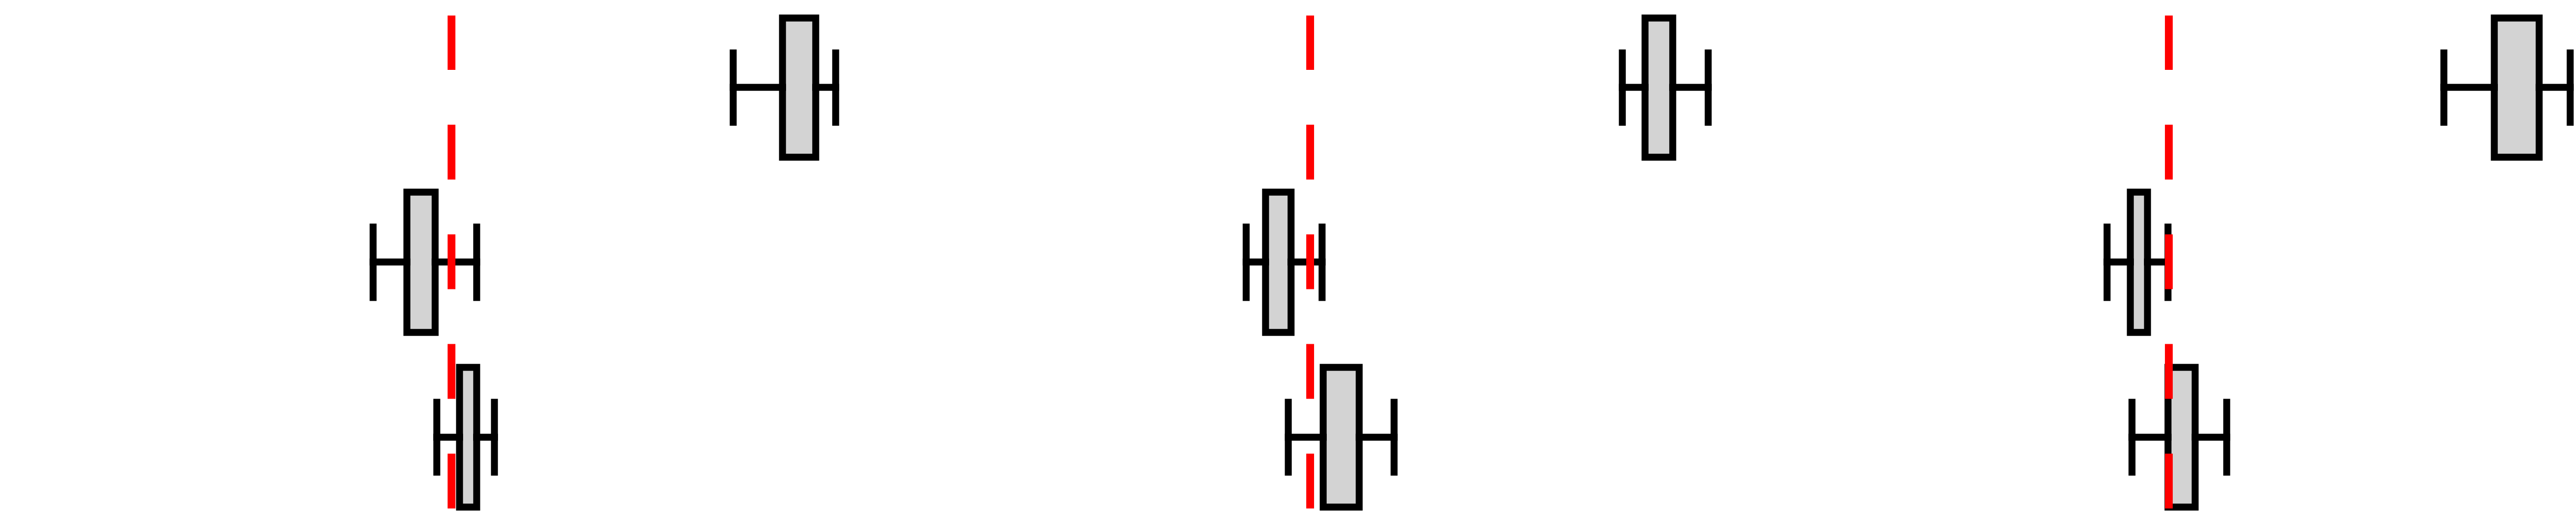
\includegraphics[width=6cm]{Figures/boxplots_model1_priorbroad.png}}} & \multicolumn{3}{c}{\multirow{3}{*}{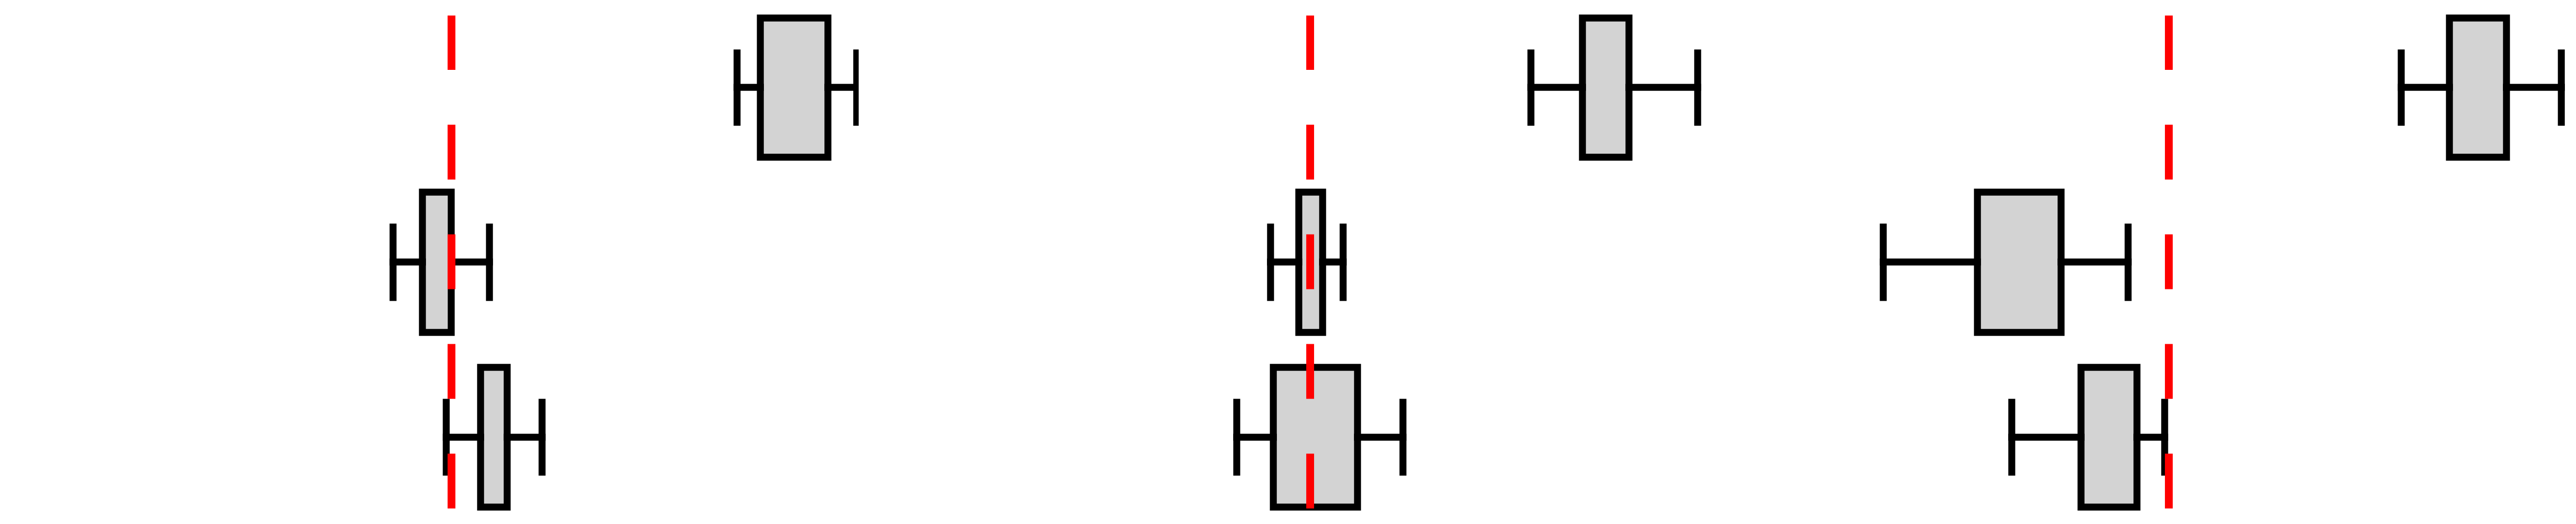
\includegraphics[width=6cm]{Figures/boxplots_model1_priornarrow.png}}} & \textbf{0.73}\\
& DE & \multicolumn{3}{c}{} & \multicolumn{3}{c}{} & \textbf{0.40}\\
& DE-SNK & \multicolumn{3}{c}{} & \multicolumn{3}{c}{} & \textbf{0.44}\\
\cmidrule(lr){1-2} \cmidrule(lr){3-5} \cmidrule(lr){6-8} \cmidrule(lr){9-9}
\multirow{3}{*}{2} & AI & \multicolumn{3}{c}{\multirow{3}{*}{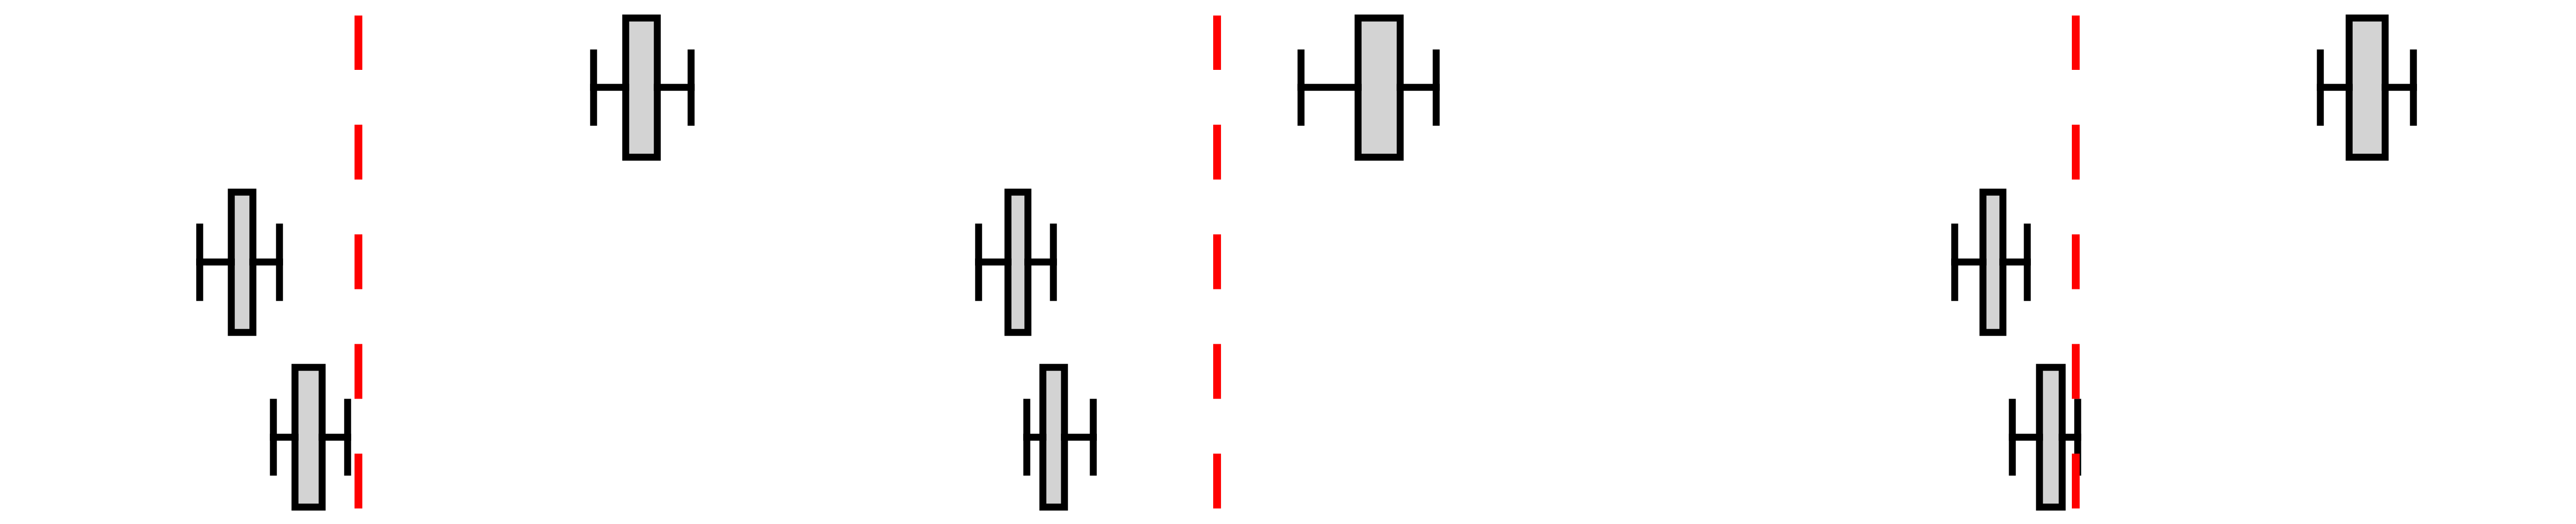
\includegraphics[width=6cm]{Figures/boxplots_model2_priorbroad.png}}} & \multicolumn{3}{c}{\multirow{3}{*}{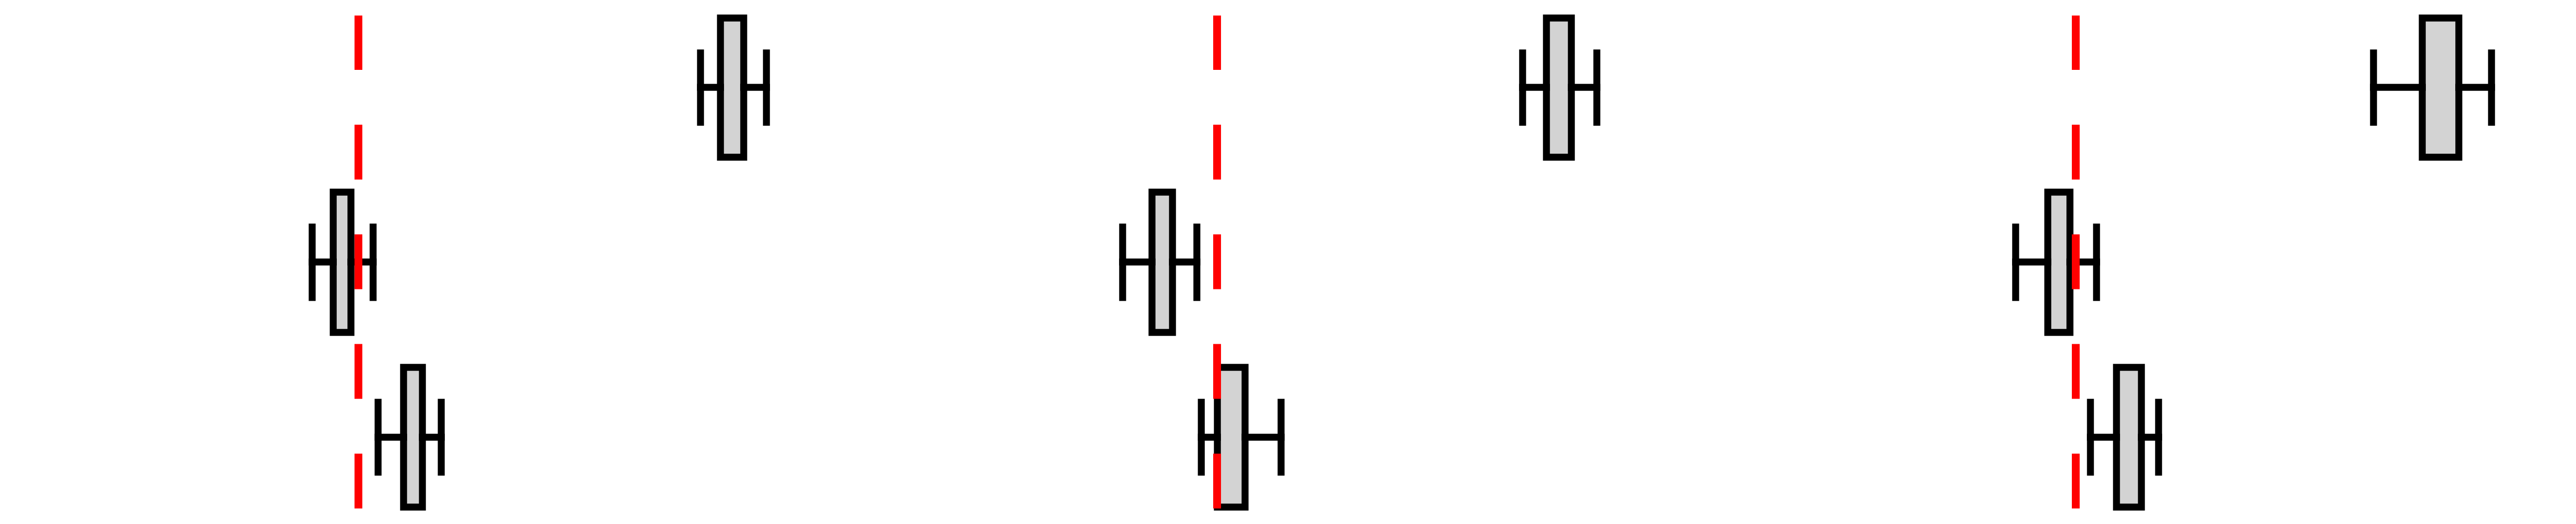
\includegraphics[width=6cm]{Figures/boxplots_model2_priornarrow.png}}} & \textbf{0.64}\\
& DE & \multicolumn{3}{c}{} & \multicolumn{3}{c}{} & \textbf{0.28}\\
& DE-SNK & \multicolumn{3}{c}{} & \multicolumn{3}{c}{} & \textbf{0.33}\\
\cmidrule(lr){1-2} \cmidrule(lr){3-5} \cmidrule(lr){6-8} \cmidrule(lr){9-9}
\multirow{3}{*}{3} & AI & \multicolumn{3}{c}{\multirow{3}{*}{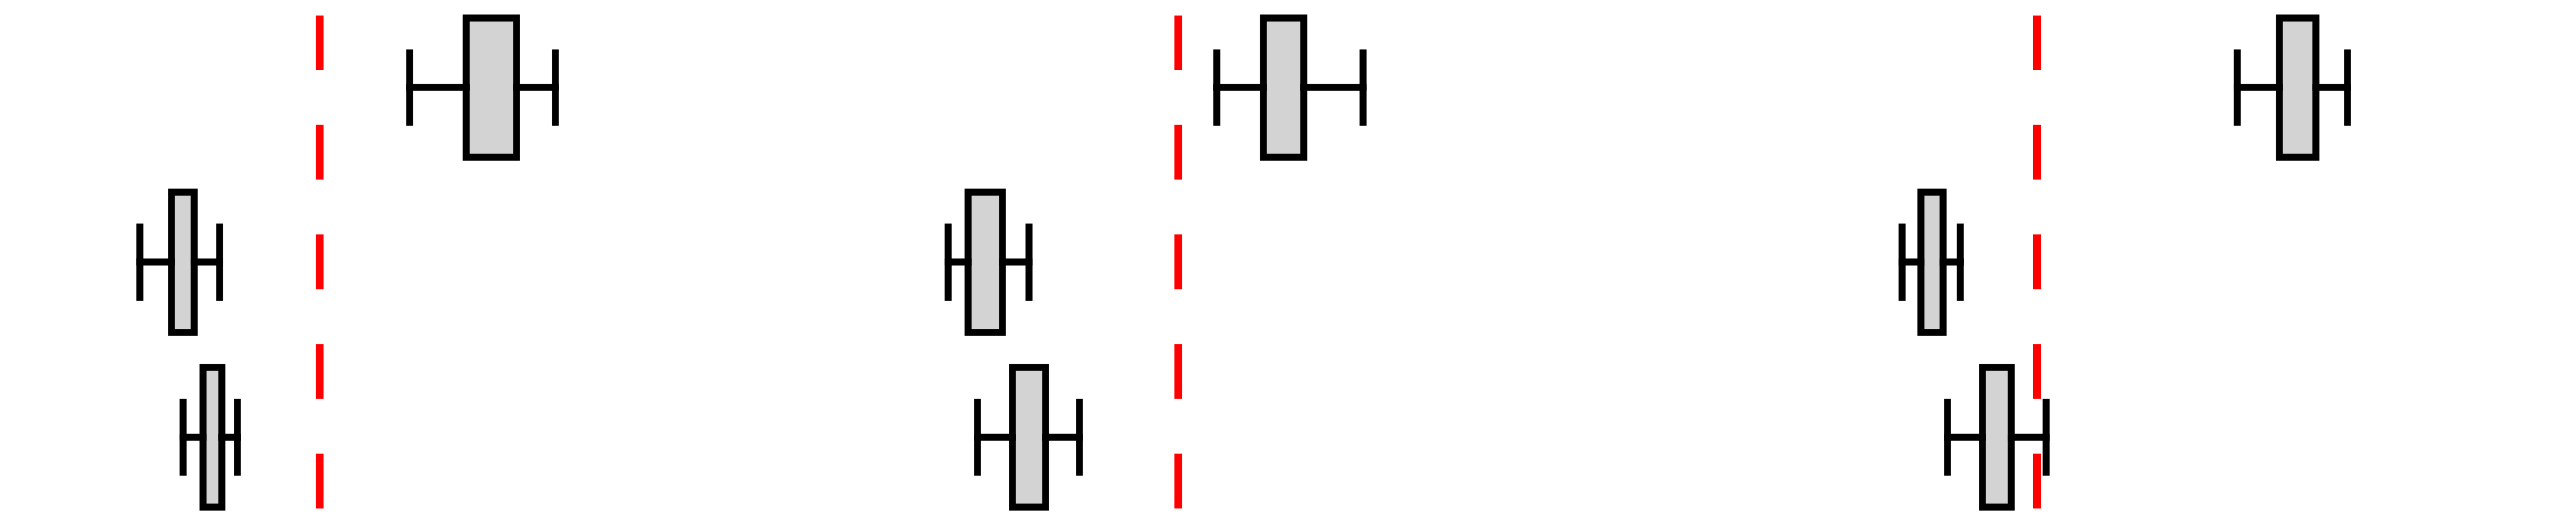
\includegraphics[width=6cm]{Figures/boxplots_model3_priorbroad.png}}} & \multicolumn{3}{c}{\multirow{3}{*}{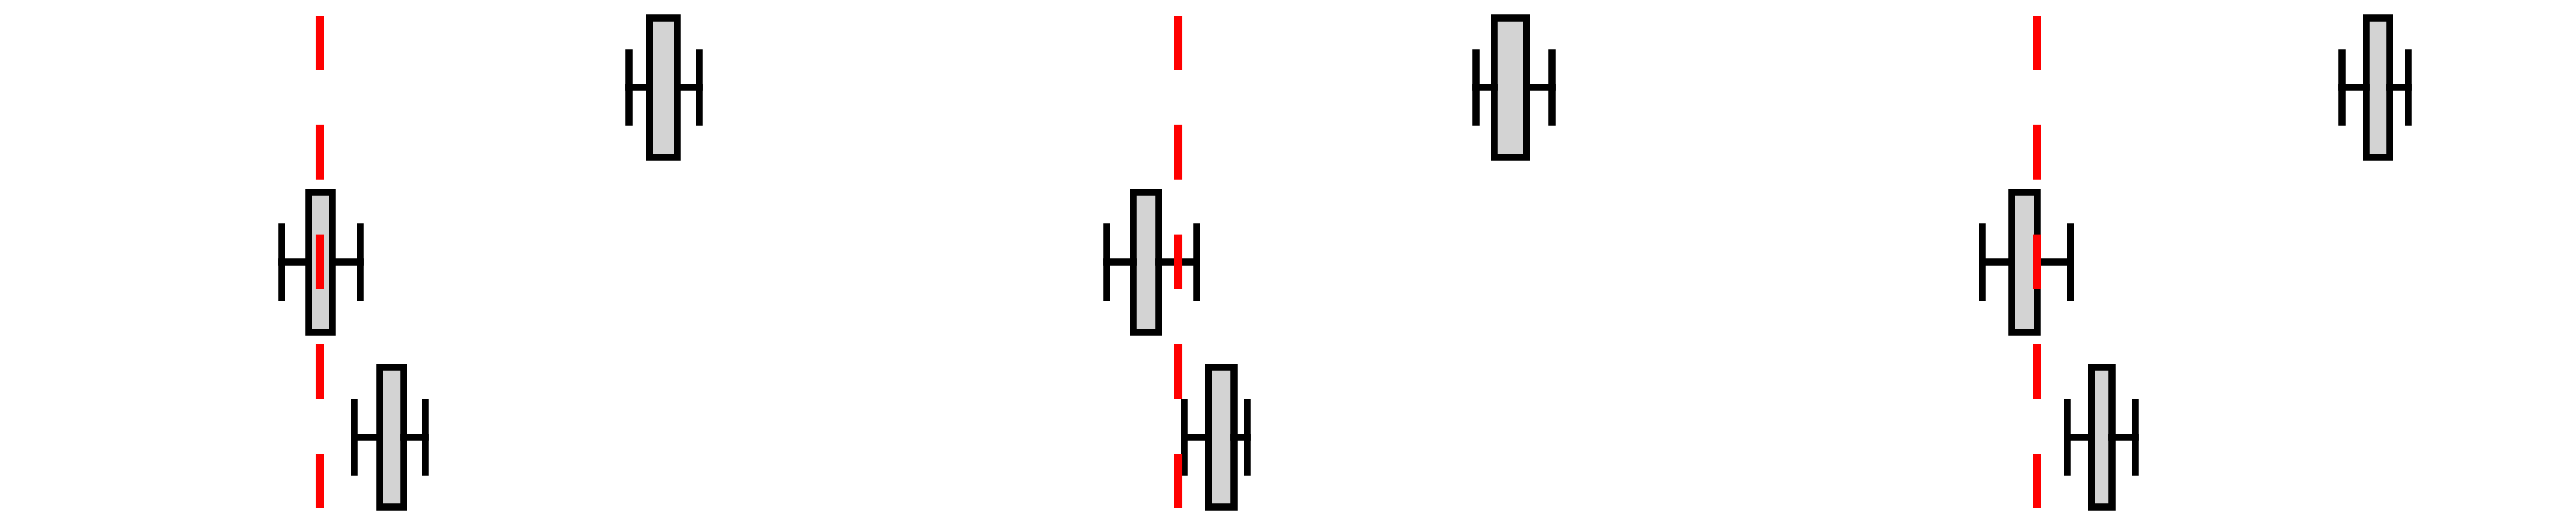
\includegraphics[width=6cm]{Figures/boxplots_model3_priornarrow.png}}} & \textbf{0.56}\\
& DE & \multicolumn{3}{c}{} & \multicolumn{3}{c}{} & \textbf{0.24}\\
& DE-SNK & \multicolumn{3}{c}{} & \multicolumn{3}{c}{} & \textbf{0.30}\\
\cmidrule(lr){1-2} \cmidrule(lr){3-5} \cmidrule(lr){6-8} \cmidrule(lr){9-9}
\multirow{3}{*}{4} & AI & \multicolumn{3}{c}{\multirow{3}{*}{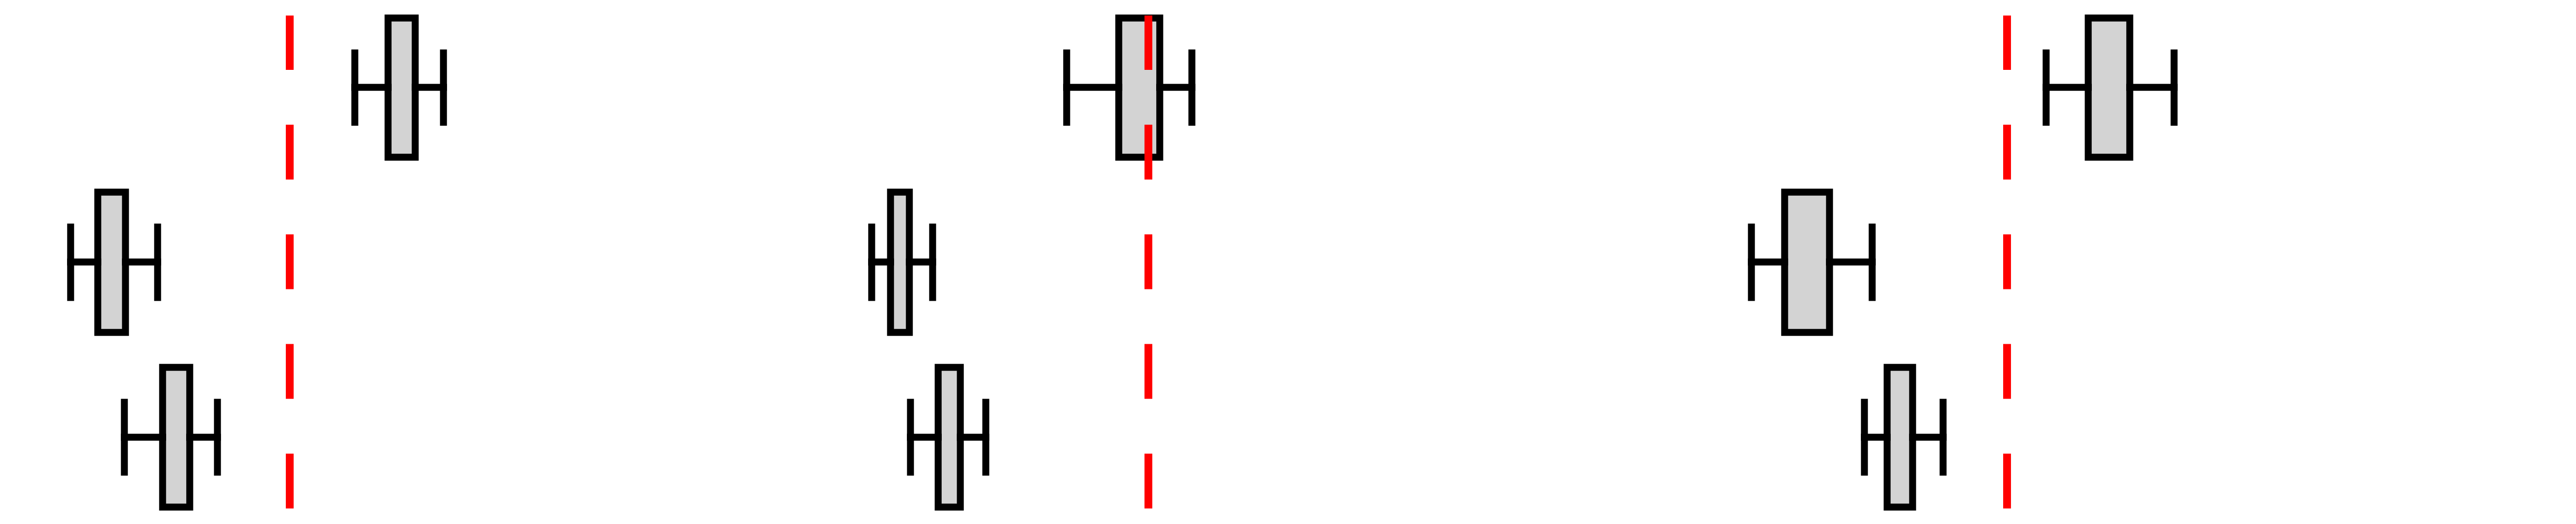
\includegraphics[width=6cm]{Figures/boxplots_model4_priorbroad.png}}} & \multicolumn{3}{c}{\multirow{3}{*}{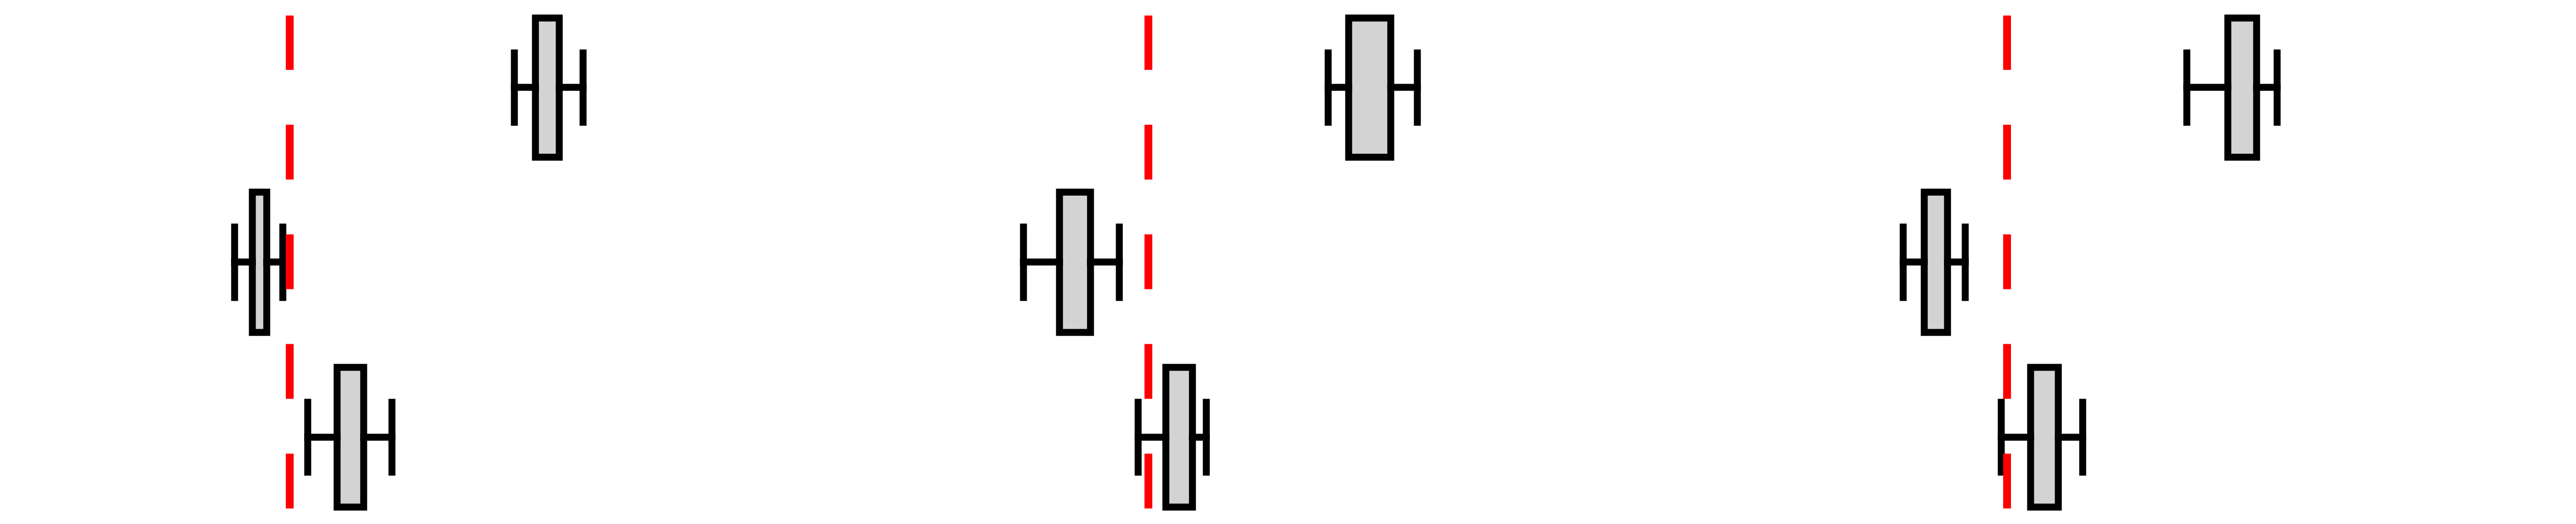
\includegraphics[width=6cm]{Figures/boxplots_model4_priornarrow.png}}} & \textbf{0.44}\\
& DE & \multicolumn{3}{c}{} & \multicolumn{3}{c}{} & \textbf{0.16}\\
& DE-SNK & \multicolumn{3}{c}{} & \multicolumn{3}{c}{} & \textbf{0.25}\\
\midrule
\multicolumn{2}{l}{\textbf{Average}} & \hspace{13pt}\textbf{0.37} & \hspace{13pt}\textbf{0.30} & \hspace{13pt}\textbf{0.38} & \hspace{13pt}\textbf{0.46} & \hspace{13pt}\textbf{0.43} & \hspace{13pt}\textbf{0.43} & \textbf{-}\\
\bottomrule
\end{tabularx}
\end{table*}

\begin{table*}[hbt]
\centering
\caption{The Estimated Effective Sample Size ($\widehat{ESS}$) for each scenario. The presented values were obtained by first calculating the mean $\widehat{ESS}$ for the last 1000 steps of each chain. Then, the sum was taken for all 10 chains of all 5 ensembles (50 chains total and 50,000 samples). For interpretability, row and column averages are also provided.}
\label{tab_ess_mean}
\begin{tabularx}{\textwidth}{llXXXXXXX}
\toprule
\multirow{2}{*}{Model} & \multirow{2}{*}{Sampler} & \multicolumn{3}{c}{Wide prior} & \multicolumn{3}{c}{Narrow prior} & \multirow{2}{*}{Average}\\
\cmidrule(lr){3-5} \cmidrule(lr){6-8} 
& & 1 obs & 3 obs & 5 obs & 1 obs & 3 obs & 5 obs & \\
\cmidrule(lr){1-2} \cmidrule(lr){3-5} \cmidrule(lr){6-8} \cmidrule(lr){9-9}
\multirow{3}{*}{1} & AI & 2462 & 2291 & 2422 & 3341 & 2878 & 3036 &  \textbf{2738} \\
& DE & 9377 & 5755 & 9241 & 7743 & 10708 & 5165 & \textbf{7998} \\
& DE-SNK & 8534 & 4637 & 8902 & 7460 & 9193 & 5212 & \textbf{7323}\\
\cmidrule(lr){1-2} \cmidrule(lr){3-5} \cmidrule(lr){6-8} \cmidrule(lr){9-9}
\multirow{3}{*}{2} & AI & 2867 & 1686 & 3009 & 4252 & 3506 & 4210 & \textbf{1567}\\
& DE & 3498 & 1801 & 4147 & 6241 & 4459 & 6508 & \textbf{4442}\\
& DE-SNK & 3840 & 1906 & 4045 & 6168 & 4278 & 5953 & \textbf{4365}\\
\cmidrule(lr){1-2} \cmidrule(lr){3-5} \cmidrule(lr){6-8} \cmidrule(lr){9-9}
\multirow{3}{*}{3} & AI & 1065 & 903 & 1276 & 1673 & 1612 & 1851 & \textbf{1397}\\
& DE & 2323 & 1629 & 2494 & 4787 & 4131 & 4393 & \textbf{3293} \\
& DE-SNK & 2585 & 1620 & 2890 & 4383 & 3706 & 4292 & \textbf{3246} \\
\cmidrule(lr){1-2} \cmidrule(lr){3-5} \cmidrule(lr){6-8} \cmidrule(lr){9-9}
\multirow{3}{*}{4} & AI & 807 & 670 & 805 & 1202 & 1094 & 1075 & \textbf{942}\\
& DE & 1333 & 851 & 1026 & 2719 & 2045 & 2063 & \textbf{1673}\\
& DE-SNK & 1514 & 921 & 1462 & 2748 & 2369 & 2326 & \textbf{1890}\\
\midrule
\textbf{Average} &  & \textbf{3228} & \textbf{1985} & \textbf{3345} & \textbf{4207} & \textbf{4015} & \textbf{3657} & - \\
\bottomrule
\end{tabularx}
\end{table*}

The estimated Effective Sample Size ($\widehat{ESS}$) decreases with increasing model number (\hyperref[tab_ess_mean]{\textcolor{blue}{Table }\ref{tab_ess_mean}}). This is what was expected based on the acceptance rate also decreasing with increasing Model number (\hyperref[tab_fracs]{\textcolor{blue}{Table }\ref{tab_fracs}}). Although AI has the highest acceptance rate, its $\widehat{ESS}$ is actually the lowest for almost all scenarios. Thus, the autocorrelation of Markov chains must be relatively high for AI, implying that the AI 'Stretch' move produces relatively poor proposals. There is no clear 

\newpage
\noindent winner for $\widehat{ESS}$, with DE and DE-SNK reporting similar values for most models, except for Model 4, for which DE-SNK consistently outperforms DE. Using more observations for likelihood evaluations appears to have a negative effect on the $\widehat{ESS}$, although not distinctly (column totals \hyperref[tab_ess_mean]{\textcolor{blue}{Table }\ref{tab_ess_mean}}). Using a more informative prior does appear to have a positive effect on the $\widehat{ESS}$ (\hyperref[tab_ess_mean]{\textcolor{blue}{Table }\ref{tab_ess_mean}}), consistent with more optimal acceptance rates for the narrow prior (\hyperref[tab_fracs]{\textcolor{blue}{Table }\ref{tab_fracs}}). % consider adding a comment about the variation between different ensembles (standard deviation presented as percentage may atleast for my analysis be valuable

\begin{table*}[ht]
\centering
\caption{The number of ensembles with all Gelman-Rubin diagnostic values ($\hat{R}$) below the threshold of 1.05. First, $\hat{R}$ was calculated for all parameters using the last 1000 steps of each chain per ensemble. Then, the ensembles with all $\hat{R} < 1.05$ were counted for each scenario. For interpretability, row and column averages are also provided.}
\label{tab_rhat_mean}
\begin{tabularx}{\textwidth}{llXXXXXXX}
\toprule
\multirow{2}{*}{Model} & \multirow{2}{*}{Move} & \multicolumn{3}{c}{Wide prior} & \multicolumn{3}{c}{Narrow prior} & \multirow{2}{*}{Average}\\
\cmidrule(lr){3-5} \cmidrule(lr){6-8}
& & 1 obs & 3 obs & 5 obs & 1 obs & 3 obs & 5 obs & \\
\midrule
\multirow{3}{*}{1} & AI & 5 & 5 & 4 & 2 & 1 & 1 & \textbf{3.00} \\
& DE & 5 & 5 & 5 & 5 & 5 & 0 & \textbf{4.17} \\
& DE-SNK & 5 & 5 & 5 & 5 & 2 & 0 & \textbf{3.67} \\
\cmidrule(lr){1-2} \cmidrule(lr){3-5} \cmidrule(lr){6-8} \cmidrule(lr){9-9}
\multirow{3}{*}{2} & AI & 0 & 0 & 1 & 4 & 2 & 2 & \textbf{1.50} \\
& DE & 5 & 4 & 5 & 5 & 5 & 5 & \textbf{4.83} \\
& DE-SNK & 5 & 3 & 5 & 5 & 5 & 5 & \textbf{4.67} \\
\cmidrule(lr){1-2} \cmidrule(lr){3-5} \cmidrule(lr){6-8} \cmidrule(lr){9-9}
\multirow{3}{*}{3} & AI & 0 & 0 & 0 & 2 & 0 & 3 & \textbf{0.83} \\
& DE & 4 & 1 & 4 & 5 & 5 & 5 & \textbf{4.00} \\
& DE-SNK 3 & 5 & 0 & 4 & 5 & 5 & 5 & \textbf{4.00} \\
\cmidrule(lr){1-2} \cmidrule(lr){3-5} \cmidrule(lr){6-8} \cmidrule(lr){9-9}
\multirow{3}{*}{4} & AI & 0 & 0 & 0 & 0 & 0 & 0 & \textbf{0.00} \\
& DE & 0 & 0 & 0 & 5 & 1 & 4 & \textbf{1.67} \\
& DE-SNK & 1 & 0 & 0 & 5 & 5 & 4 & \textbf{2.50} \\
\midrule
\textbf{Average} & & \textbf{2.92} & \textbf{1.92} & \textbf{2.75} & \textbf{4.00} & \textbf{3.00} & \textbf{2.83} & \textbf{-} \\
\bottomrule
\end{tabularx}
\end{table*}

Too few ensembles passed the recommended $\hat{R}$ threshold of 1.01 by \cite{vehtari2021rank} for any meaningful comparison. Therefore, the threshold in \hyperref[tab_rhat_mean]{\textcolor{blue}{Table }\ref{tab_rhat_mean}} was relaxed to 1.05, which is still relatively strict compared to the original recommendation of 1.10 by \cite{gelman1992inference}. AI reports the fewest ensembles with all $\hat{R}$ below the threshold of 1.05 for each model, suggesting that AI convergences relatively poorly (\hyperref[tab_rhat_mean]{\textcolor{blue}{Table }\ref{tab_rhat_mean}}). This aligns with AI reporting the lowest $\widehat{ESS}$ values, as chains tend to have a longer integrated autocorrelation time ($\tau_f$) during burn-in \citep{hogg2018data}. Using the narrow prior results in more ensembles with all $\hat{R}$ below the threshold for Model 2,3 and 4, indicating improved convergence. This trend is consistent with $\widehat{ESS}$ being larger for Model 2,3 and 4, when using the narrow prior (\hyperref[tab_ess_mean]{\textcolor{blue}{Table }\ref{tab_ess_mean}}). For models with more parameters (higher model number), $\hat{R}$ indicates worse convergence for all samplers (\hyperref[tab_rhat_mean]{\textcolor{blue}{Table }\ref{tab_rhat_mean}}).

The median parameter values of all steps of all chains of all (5) ensembles for a scenario (from now on referred to as simply the median), are extremely similar for the different samplers  (\hyperref[tab_median_color]{\textcolor{blue}{Table }\ref{tab_median_color}}), even though AI showed the worst acceptance rate, $\widehat{ESS}$ and $\hat{R}$. The median is a much better estimate of the true parameter values ($\theta_{n,\,true}$) when using the narrow prior, opposed to using the wide prior. This difference is especially striking for parameters with a low $\theta_{n,\,true}$. Increasing the number of observations for evaluating the likelihood clearly improves the estimate of $\theta_{n,\,true}$, which is again most striking for parameters with a low $\theta_{n,\,true}$. Interestingly, using more observations was shown to decrease convergence, yet the estimate of $\theta_{n,\,true}$ improves. This suggests that using more observations leads to a better estimate of the true posterior at the cost of a longer burn-in time. 

The influence of the prior on the shape of the posterior appears strong, with the wide prior resulting in a much broader posterior (\hyperref[fig_kde_model1_DEsnooker]{\textcolor{blue}{Figure }\ref{fig_kde_model1_DEsnooker}}). These Kernel Density Estimate (KDE) plots also reveal a second mode for $\theta_1$ of Model 1, though it contains comparatively little density. Interestingly, the second optimum is (visually) absent for the scenario, where the wide prior is used in combination with three observations for evaluating the likelihood.  \hyperref[fig_kde_model1_DEsnooker]{\textcolor{blue}{Figure }\ref{fig_kde_model1_DEsnooker}} only shows results for DE-SNK, but plots for AI and DE reveal very similar posteriors (appendix figures \ref{fig_kde_model1_Stretch} and \ref{fig_kde_model1_DE}), which is consistent with \hyperref[tab_median_color]{\textcolor{blue}{Table }\ref{tab_median_color}} showing little variation of the Median from different samplers.  

Pairs plots were created for Model 2-4 to identify the posterior distributions and parameter covariances. For conciseness, pairs plots are limited to the scenario with the wide prior and 1 observation per layer. Additionally, only pairs plots for DE-SNK are shown, as different samplers produced similar pairs plots (\hyperref[additional_results]{\textcolor{blue}{Appendix }\ref{sub_pairsplots}}).  

For Model 2, both parameters show a strongly skewed unimodal distribution (\hyperref[fig_kde_model2_DEsnooker]{\textcolor{blue}{Figure }\ref{fig_kde_model2_DEsnooker}}), with the posterior of the upper layer, $\text{p}(\theta_1 | \text{data})$, being much narrower than $\text{p}(\theta_2 | \text{data})$. The joint distribution reveals that $\theta_1$ is largely insensitive to $\theta_2$, if $\theta_2 \lessapprox 0$.  

\begin{table*}[ht]
\centering
\caption{Median parameter values of all (5) ensembles, with $\theta_n$ representing the hydraulic conductivity (m/d) of layer $n$. The true hydraulic conductivities are given between parentheses in column two (Parameter). Each coloured cell represents a scenario (for which 5 ensembles were run), described by the row and column labels. The colour of each cell is an indication of how much the cell value differs from the true hydraulic conductivity of the respective layer (absolute log difference), with dark green representing no difference (best) and red representing large differences (worst). The absolute log difference was used to determine cell colours, because different parameters are of different orders of magnitude.}
\label{tab_median_color}
\begin{tabularx}{\textwidth}{lllXXXXXX}
\toprule
\multirow{2}{*}{Model} & \multirow{2}{*}{Parameter} & \multirow{2}{*}{Move} & \multicolumn{3}{c}{Wide prior} & \multicolumn{3}{c}{Narrow prior} \\
\cmidrule(lr){4-6} \cmidrule(lr){7-9}
& & & 1 obs & 3 obs & 5 obs & 1 obs & 3 obs & 5 obs \\
\midrule
\multirow{3}{*}{1} & \multirow{3}{*}{$\theta_1 \:\: (5.0)$} & AI & 13 \cellcolor[HTML]{C8E300} & 4.1 \cellcolor[HTML]{289300} & 19 \cellcolor[HTML]{FFE400} & 2.2 \cellcolor[HTML]{A8D300} & 2.7 \cellcolor[HTML]{80BF00} & 3.1 \cellcolor[HTML]{61B000} \\
& & DE & 12 \cellcolor[HTML]{C0DF00} & 4.1 \cellcolor[HTML]{2A9400} & 20 \cellcolor[HTML]{FFD800} & 2.3 \cellcolor[HTML]{A6D200} & 2.8 \cellcolor[HTML]{79BC00} & 3.0 \cellcolor[HTML]{68B300} \\
& & DE-SNK & 12 \cellcolor[HTML]{BCDD00} & 4.0 \cellcolor[HTML]{2C9500} & 19 \cellcolor[HTML]{FFE800} & 2.2 \cellcolor[HTML]{A8D300} & 2.7 \cellcolor[HTML]{7EBE00} & 3.1 \cellcolor[HTML]{64B100} \\
\cmidrule(lr){1-3} \cmidrule(lr){4-6} \cmidrule(lr){7-9}
\multirow{6}{*}{2} & \multirow{3}{*}{$\theta_1 \:\: (2.0)$} & AI & 1.9 \cellcolor[HTML]{0A8400} & 1.9 \cellcolor[HTML]{0E8600} & 2.9 \cellcolor[HTML]{49A400} & 1.3 \cellcolor[HTML]{54A900} & 1.4 \cellcolor[HTML]{41A000} & 1.9 \cellcolor[HTML]{068200} \\
& & DE & 2.0 \cellcolor[HTML]{008000} & 2.0 \cellcolor[HTML]{008000} & 2.9 \cellcolor[HTML]{4CA500} & 1.4 \cellcolor[HTML]{4EA600} & 1.4 \cellcolor[HTML]{46A200} & 1.9 \cellcolor[HTML]{068200} \\
& & DE-SNK & 2.0 \cellcolor[HTML]{008000} & 1.9 \cellcolor[HTML]{088300} & 2.9 \cellcolor[HTML]{4CA500} & 1.3 \cellcolor[HTML]{51A800} & 1.4 \cellcolor[HTML]{44A100} & 1.9 \cellcolor[HTML]{088300} \\
\cmidrule(lr){4-6} \cmidrule(lr){7-9}
& \multirow{3}{*}{$\theta_2 \:\: (1.0)$} & AI & 0.92 \cellcolor[HTML]{108700} & 1.0 \cellcolor[HTML]{008000} & 0.46 \cellcolor[HTML]{A2D000} & 1.3 \cellcolor[HTML]{3A9C00} & 1.4 \cellcolor[HTML]{49A400} & 1.4 \cellcolor[HTML]{409F00} \\
& & DE & 0.83 \cellcolor[HTML]{269200} & 0.86 \cellcolor[HTML]{208F00} & 0.54 \cellcolor[HTML]{80BF00} & 1.3 \cellcolor[HTML]{3A9C00} & 1.4 \cellcolor[HTML]{4CA500} & 1.4 \cellcolor[HTML]{46A200} \\
& & DE-SNK & 0.79 \cellcolor[HTML]{309700} & 0.96 \cellcolor[HTML]{088300} & 0.57 \cellcolor[HTML]{76BA00} & 1.3 \cellcolor[HTML]{3A9C00} & 1.4 \cellcolor[HTML]{49A400} & 1.4 \cellcolor[HTML]{48A300} \\
\cmidrule(lr){1-3} \cmidrule(lr){4-6} \cmidrule(lr){7-9}
\multirow{9}{*}{3} & \multirow{3}{*}{$\theta_1 \:\: (1.0)$} & AI & 0.90 \cellcolor[HTML]{148900} & 0.89 \cellcolor[HTML]{188B00} & 1.3 \cellcolor[HTML]{309700} & 1.1 \cellcolor[HTML]{168A00} & 0.89 \cellcolor[HTML]{168A00} & 1.2 \cellcolor[HTML]{229000} \\
& & DE & 0.83 \cellcolor[HTML]{269200} & 0.84 \cellcolor[HTML]{249100} & 1.2 \cellcolor[HTML]{2E9600} & 1.1 \cellcolor[HTML]{168A00} & 0.90 \cellcolor[HTML]{148900} & 1.2 \cellcolor[HTML]{269200} \\
& & DE-SNK & 0.79 \cellcolor[HTML]{329800} & 0.77 \cellcolor[HTML]{389B00} & 1.3 \cellcolor[HTML]{3A9C00} & 1.1 \cellcolor[HTML]{148900} & 0.91 \cellcolor[HTML]{148900} & 1.2 \cellcolor[HTML]{229000} \\
\cmidrule(lr){4-6} \cmidrule(lr){7-9}
& \multirow{3}{*}{$\theta_2 \:\: (0.010)$} & AI & 0.048 \cellcolor[HTML]{FFB200} & 0.089 \cellcolor[HTML]{FF3400} & 0.0087 \cellcolor[HTML]{1C8D00} & 0.010 \cellcolor[HTML]{028000} & 0.010 \cellcolor[HTML]{068200} & 0.0095 \cellcolor[HTML]{0A8400} \\
& & DE & 0.047 \cellcolor[HTML]{FFB800} & 0.090 \cellcolor[HTML]{FF3000} & 0.0088 \cellcolor[HTML]{188B00} & 0.010 \cellcolor[HTML]{028000} & 0.010 \cellcolor[HTML]{048100} & 0.0093 \cellcolor[HTML]{0E8600} \\
& & DE-SNK & 0.053 \cellcolor[HTML]{FFA200} & 0.092 \cellcolor[HTML]{FF2900} & 0.0083 \cellcolor[HTML]{269200} & 0.010 \cellcolor[HTML]{068200} & 0.010 \cellcolor[HTML]{048100} & 0.0095 \cellcolor[HTML]{0A8400} \\
\cmidrule(lr){4-6} \cmidrule(lr){7-9}
& \multirow{3}{*}{$\theta_3 \:\: (10)$} & AI & 6.1 \cellcolor[HTML]{66B200} & 3.1 \cellcolor[HTML]{F8FB00} & 16 \cellcolor[HTML]{60AF00} & 11 \cellcolor[HTML]{0A8400} & 8.6 \cellcolor[HTML]{1E8E00} & 10 \cellcolor[HTML]{088300} \\
& & DE & 6.9 \cellcolor[HTML]{4EA600} & 3.2 \cellcolor[HTML]{F0F700} & 15 \cellcolor[HTML]{50A700} & 10 \cellcolor[HTML]{048100} & 8.7 \cellcolor[HTML]{1C8D00} & 10 \cellcolor[HTML]{028000} \\
& & DE-SNK & 6.0 \cellcolor[HTML]{6CB500} & 3.4 \cellcolor[HTML]{E2F000} & 15 \cellcolor[HTML]{56AA00} & 10 \cellcolor[HTML]{028000} & 8.7 \cellcolor[HTML]{1E8E00} & 10 \cellcolor[HTML]{088300} \\
\cmidrule(lr){1-3} \cmidrule(lr){4-6} \cmidrule(lr){7-9}
\multirow{15}{*}{4} & \multirow{3}{*}{$\theta_1 \:\: (1.0)$} & AI & 1.9 \cellcolor[HTML]{83C100} & 1.2 \cellcolor[HTML]{2C9500} & 0.95 \cellcolor[HTML]{0A8400} & 2.1 \cellcolor[HTML]{98CB00} & 2.3 \cellcolor[HTML]{B0D700} & 1.6 \cellcolor[HTML]{64B100} \\
& & DE & 2.0 \cellcolor[HTML]{8CC500} & 1.2 \cellcolor[HTML]{269200} & 0.90 \cellcolor[HTML]{148900} & 2.1 \cellcolor[HTML]{96CA00} & 2.3 \cellcolor[HTML]{B0D700} & 1.6 \cellcolor[HTML]{68B300} \\
& & DE-SNK & 2.0 \cellcolor[HTML]{90C700} & 1.1 \cellcolor[HTML]{148900} & 0.96 \cellcolor[HTML]{068200} & 2.1 \cellcolor[HTML]{98CB00} & 2.3 \cellcolor[HTML]{B2D800} & 1.7 \cellcolor[HTML]{69B400} \\
\cmidrule(lr){4-6} \cmidrule(lr){7-9}
& \multirow{3}{*}{$\theta_2 \:\: (0.10)$} & AI & 0.020 \cellcolor[HTML]{FFB000} & 0.095 \cellcolor[HTML]{0A8400} & 0.067 \cellcolor[HTML]{54A900} & 0.11 \cellcolor[HTML]{0E8600} & 0.11 \cellcolor[HTML]{108700} & 0.072 \cellcolor[HTML]{46A200} \\
& & DE & 0.021 \cellcolor[HTML]{FFB200} & 0.075 \cellcolor[HTML]{3C9D00} & 0.067 \cellcolor[HTML]{54A900} & 0.11 \cellcolor[HTML]{0E8600} & 0.11 \cellcolor[HTML]{108700} & 0.070 \cellcolor[HTML]{49A400} \\
& & DE-SNK & 0.019 \cellcolor[HTML]{FFA200} & 0.063 \cellcolor[HTML]{60AF00} & 0.064 \cellcolor[HTML]{5CAD00} & 0.11 \cellcolor[HTML]{0E8600} & 0.11 \cellcolor[HTML]{128800} & 0.069 \cellcolor[HTML]{4CA500} \\
\cmidrule(lr){4-6} \cmidrule(lr){7-9}
& \multirow{3}{*}{$\theta_3 \:\: (4.0)$} & AI & 6.6 \cellcolor[HTML]{68B300} & 2.9 \cellcolor[HTML]{41A000} & 3.1 \cellcolor[HTML]{389B00} & 1.3 \cellcolor[HTML]{EEF600} & 1.3 \cellcolor[HTML]{EAF400} & 1.8 \cellcolor[HTML]{A8D300} \\
& & DE & 5.7 \cellcolor[HTML]{49A400} & 3.2 \cellcolor[HTML]{2A9400} & 3.8 \cellcolor[HTML]{0A8400} & 1.3 \cellcolor[HTML]{EEF600} & 1.3 \cellcolor[HTML]{EAF400} & 1.8 \cellcolor[HTML]{ACD500} \\
& & DE-SNK & 5.9 \cellcolor[HTML]{50A700} & 4.0 \cellcolor[HTML]{008000} & 3.2 \cellcolor[HTML]{2A9400} & 1.3 \cellcolor[HTML]{F2F800} & 1.3 \cellcolor[HTML]{ECF500} & 1.8 \cellcolor[HTML]{ACD500} \\
\cmidrule(lr){4-6} \cmidrule(lr){7-9}
& \multirow{3}{*}{$\theta_4 \:\: (0.010)$} & AI & 0.068 \cellcolor[HTML]{FF6900} & 0.078 \cellcolor[HTML]{FF4E00} & 0.019 \cellcolor[HTML]{82C000} & 0.010 \cellcolor[HTML]{028000} & 0.012 \cellcolor[HTML]{229000} & 0.011 \cellcolor[HTML]{0C8500} \\
& & DE & 0.049 \cellcolor[HTML]{FFB200} & 0.099 \cellcolor[HTML]{FF1C00} & 0.017 \cellcolor[HTML]{74B900} & 0.010 \cellcolor[HTML]{048100} & 0.012 \cellcolor[HTML]{249100} & 0.010 \cellcolor[HTML]{028000} \\
& & DE-SNK & 0.059 \cellcolor[HTML]{FF8A00} & 0.11 \cellcolor[HTML]{FF0000} & 0.018 \cellcolor[HTML]{79BC00} & 0.010 \cellcolor[HTML]{068200} & 0.012 \cellcolor[HTML]{1E8E00} & 0.010 \cellcolor[HTML]{008000} \\
\cmidrule(lr){4-6} \cmidrule(lr){7-9}
& \multirow{3}{*}{$\theta_5 \:\: (3.0)$} & AI & 7.8 \cellcolor[HTML]{CAE400} & 2.4 \cellcolor[HTML]{2C9500} & 5.5 \cellcolor[HTML]{7EBE00} & 1.2 \cellcolor[HTML]{BADC00} & 1.2 \cellcolor[HTML]{C8E300} & 1.8 \cellcolor[HTML]{6CB500} \\
& & DE & 9.0 \cellcolor[HTML]{E8F300} & 2.7 \cellcolor[HTML]{128800} & 4.8 \cellcolor[HTML]{64B100} & 1.2 \cellcolor[HTML]{BCDD00} & 1.1 \cellcolor[HTML]{CAE400} & 1.7 \cellcolor[HTML]{74B900} \\
& & DE-SNK & 11 \cellcolor[HTML]{FFEE00} & 3.0 \cellcolor[HTML]{028000} & 5.3 \cellcolor[HTML]{74B900} & 1.2 \cellcolor[HTML]{BCDD00} & 1.1 \cellcolor[HTML]{D0E700} & 1.7 \cellcolor[HTML]{74B900} \\
\bottomrule
\end{tabularx}
\end{table*}

\newpage
The parameters of Model 3 show more symmetric behaviour, with $\text{p}(\theta_1 | \text{data})$ again being the most concentrated (\hyperref[fig_kde_model3_DEsnooker]{\textcolor{blue}{Figure }\ref{fig_kde_model3_DEsnooker}}). Another interesting feature of $\text{p}(\theta_1 | \text{data})$ is that it is approximately uniform (though it does appear to have a mode on the right side). In reality, the distribution may look even more uniform with sharper edges, due to KDE having the (negative) effect of smoothing vertical edges, giving the appearance of tails \citep{analytica_kde}.
\begin{figure*}[htb]
\centering
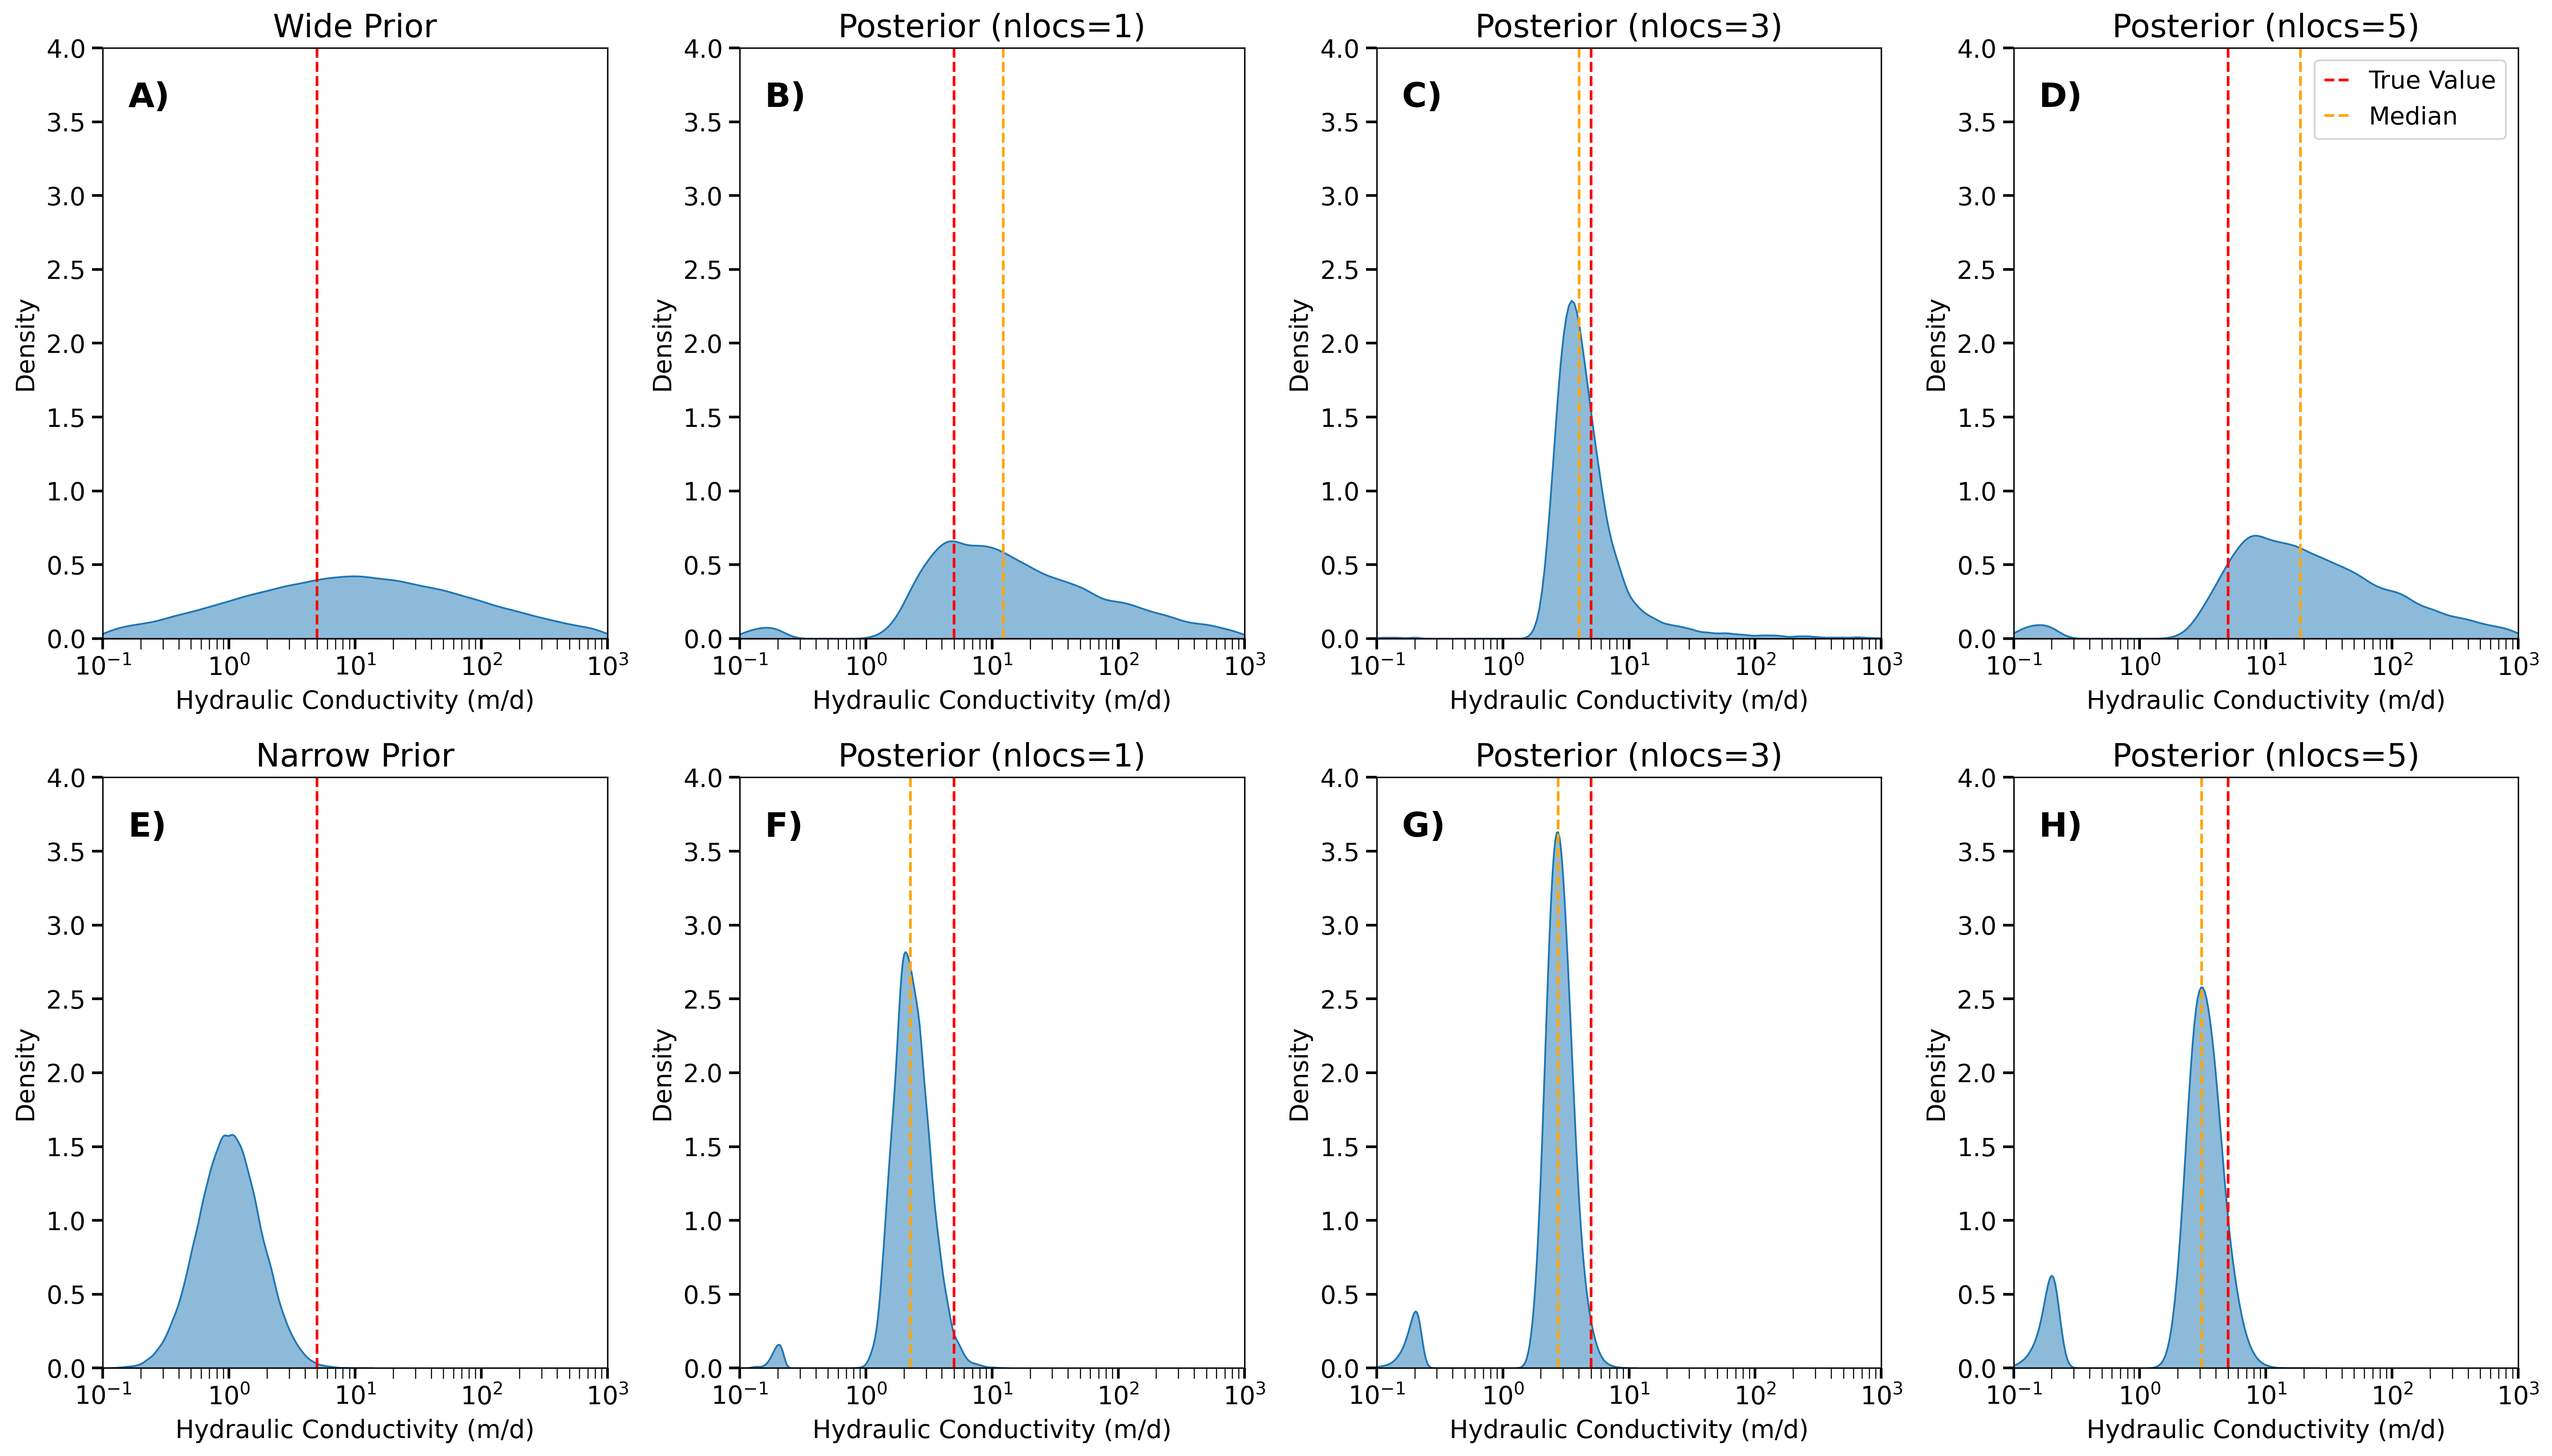
\includegraphics[width=1.0\textwidth]{Figures/kde_model1_DEsnooker.png}
\caption{Kernel Density Estimate plots for the only parameter of Model 1 ($\theta_1$), which was calibrated with DE-SNK. \textbf{A)} shows the wide prior. \textbf{B), C)} and \textbf{D)} show the posteriors after calibrating $\theta_1$ with: the wide prior in combination with 1,3 or 5 observations for evaluating the likelihood, respectively. Similarly, \textbf{E)} shows the narrow prior. \textbf{F), G)} and \textbf{H)} show the posteriors after calibrating $\theta_1$ with: the narrow prior in combination with 1,3 or 5 observations for evaluating the likelihood. In each plot the dashed red line indicates the true value for $\theta_1$. Similarly, the posterior median is indicated by a dashed yellow line.}\label{fig_kde_model1_DEsnooker}
\end{figure*}
\begin{figure}[htb]
\centering
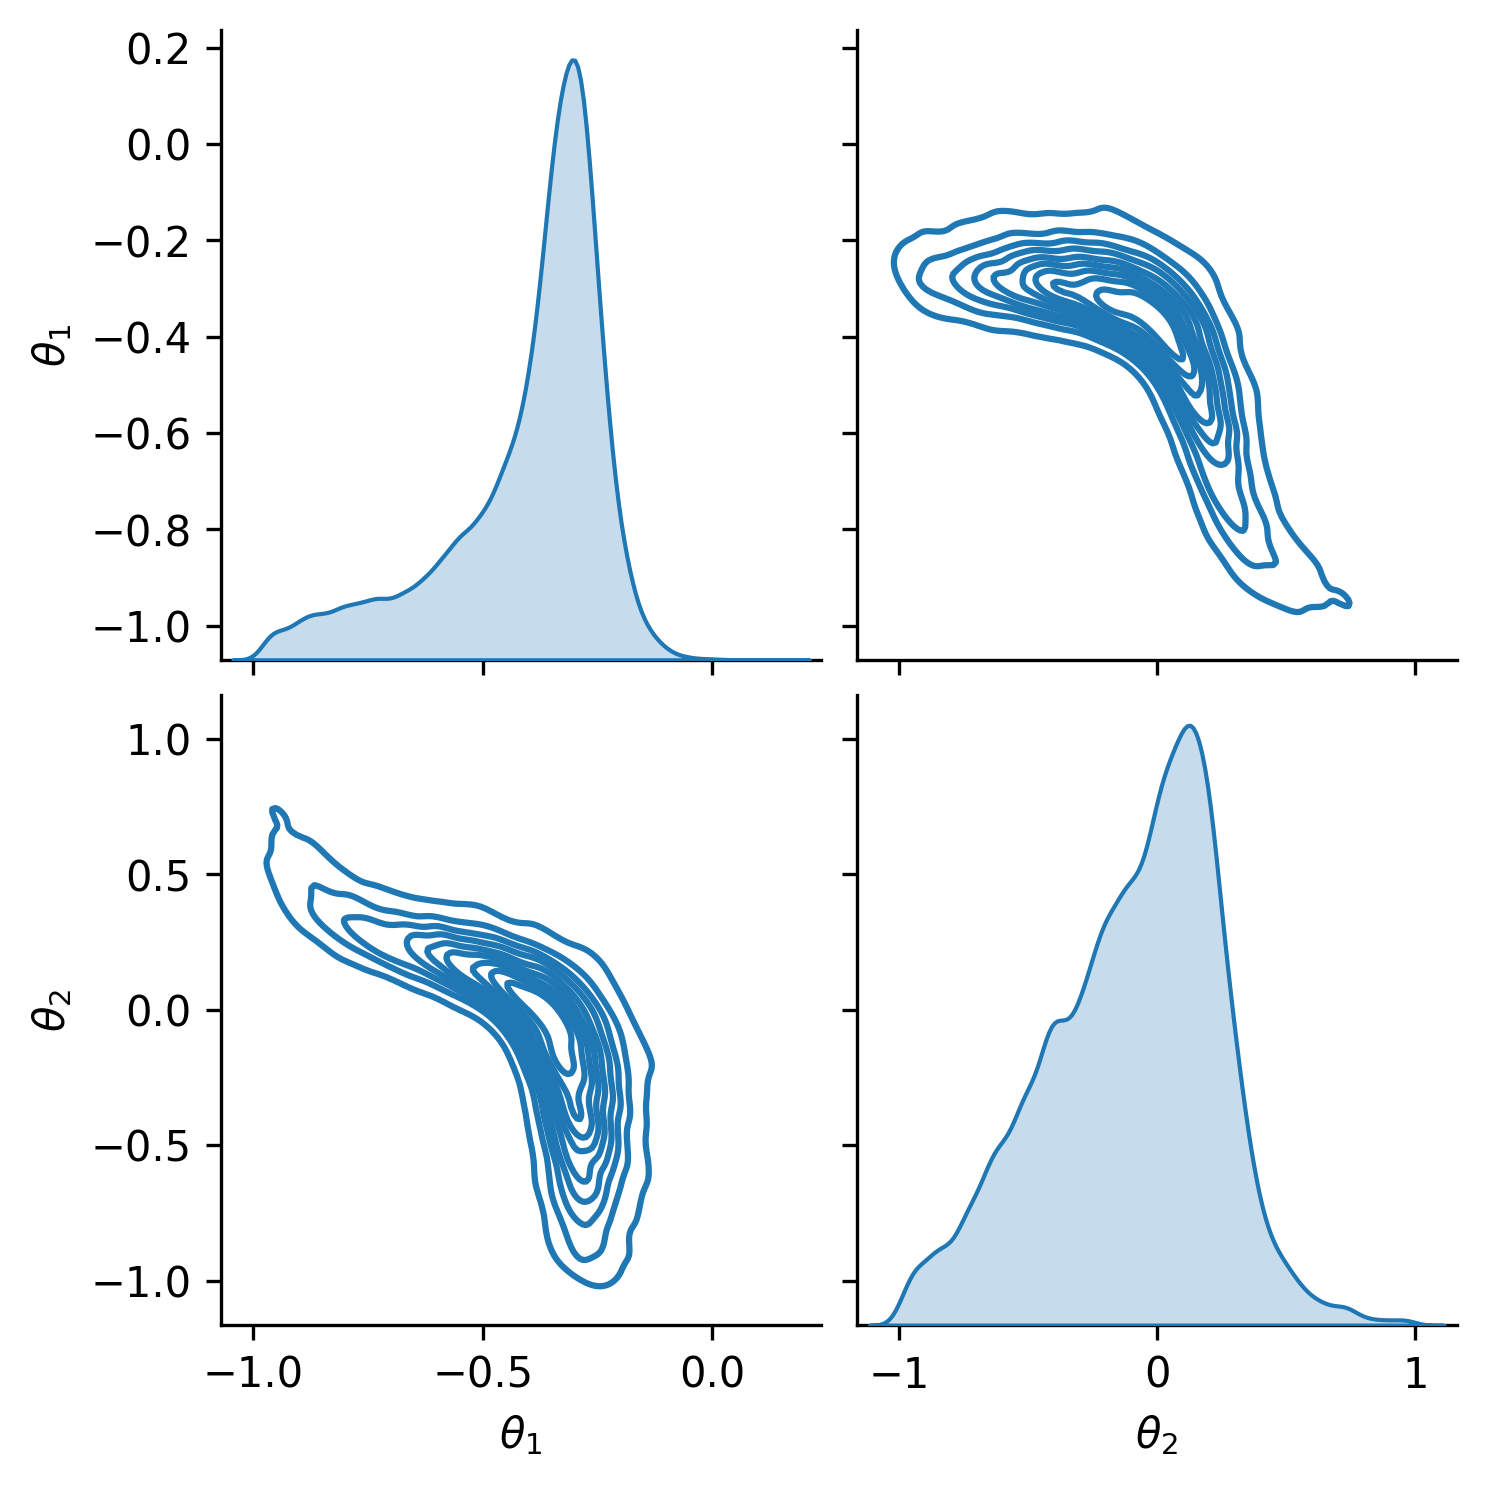
\includegraphics[width=0.8\linewidth]{Figures/kde_model2_DEsnooker.png}
\caption{Pairs plots (with a KDE style) for all calibrated parameters of Model 2. The presented data is from 5 ensembles (last 1000 steps of each chain), run with DE-SNK, a wide prior and 1 observation for evaluating the likelihood. The parameters as presented here are untransformed (used for MCMC). }\label{fig_kde_model2_DEsnooker}
\end{figure}
\begin{figure}[htb]
\centering
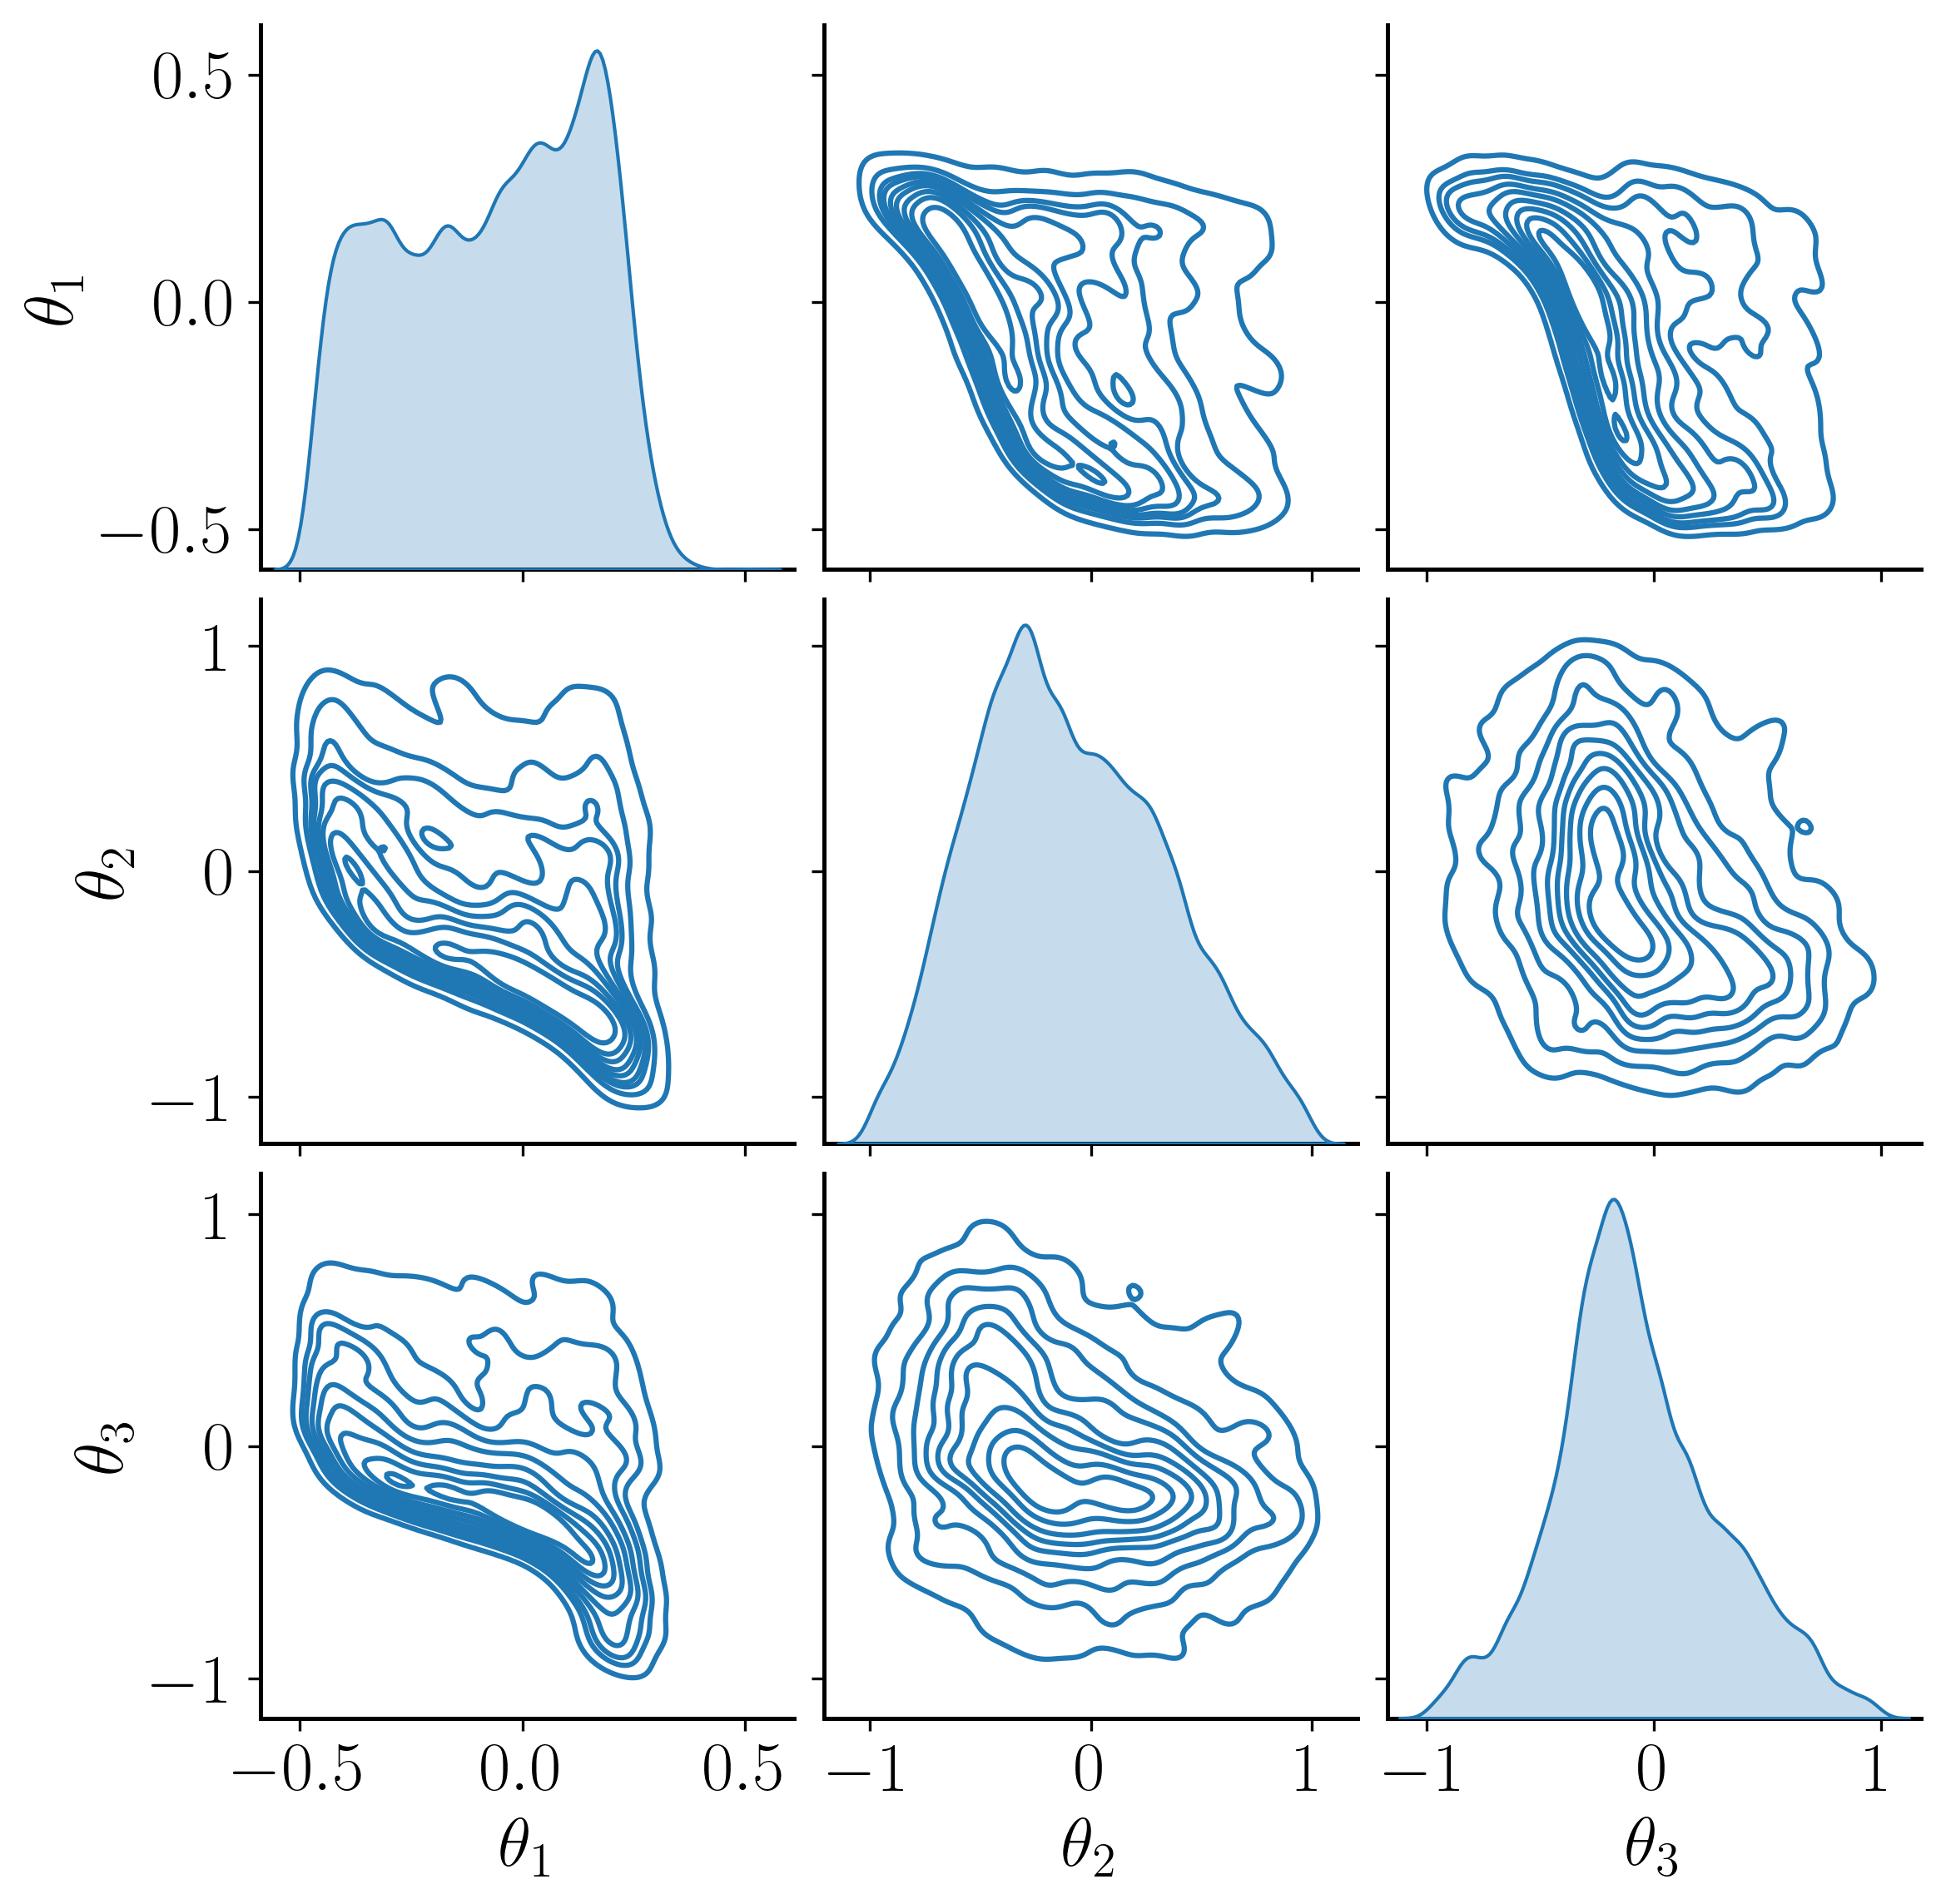
\includegraphics[width=0.8\linewidth]{Figures/kde_model3_DEsnooker.png}
\caption{Pairs plots (with a KDE style) for all calibrated parameters of Model 3. The presented data is from 5 ensembles (last 1000 steps of each chain), run with DE-SNK, a wide prior and 1 observation for evaluating the likelihood. The parameters as presented here are untransformed (used for MCMC).}\label{fig_kde_model3_DEsnooker}
\end{figure}
\FloatBarrier
\clearpage
\noindent Joint distributions indicate an inversely proportional relationship between $\theta_1$ and the other two parameters (\hyperref[fig_kde_model3_DEsnooker]{\textcolor{blue}{Figure }\ref{fig_kde_model3_DEsnooker}}). The approximately spherical joint distribution of $\theta_2$ and $\theta_3$ suggests that these parameters are insensitive to one another \citep{gelman2021bayesian}.  

For Model 4, $\text{p}(\theta_1 | \text{data})$ is the most concentrated posterior (\hyperref[fig_kde_model4_DEsnooker]{\textcolor{blue}{Figure }\ref{fig_kde_model4_DEsnooker}}), similar to Models 2 and 3. All posteriors are unimodal, with $\text{p}(\theta_1 | \text{data})$ and $\text{p}(\theta_2 | \text{data})$ being skewed, while the other posteriors appear symmetric. Joint distributions reveal that the parameters of the deeper layers ($\theta_3$, $\theta_4$, $\theta_5$) are insensitive to one another, with their posteriors increasingly resembling the prior distribution, as the parameter number increases (see the narrow prior in \hyperref[fig_kde_model1_DEsnooker]{\textcolor{blue}{Figure }\ref{fig_kde_model1_DEsnooker}}).

\begin{figure}[htb!]
\centering
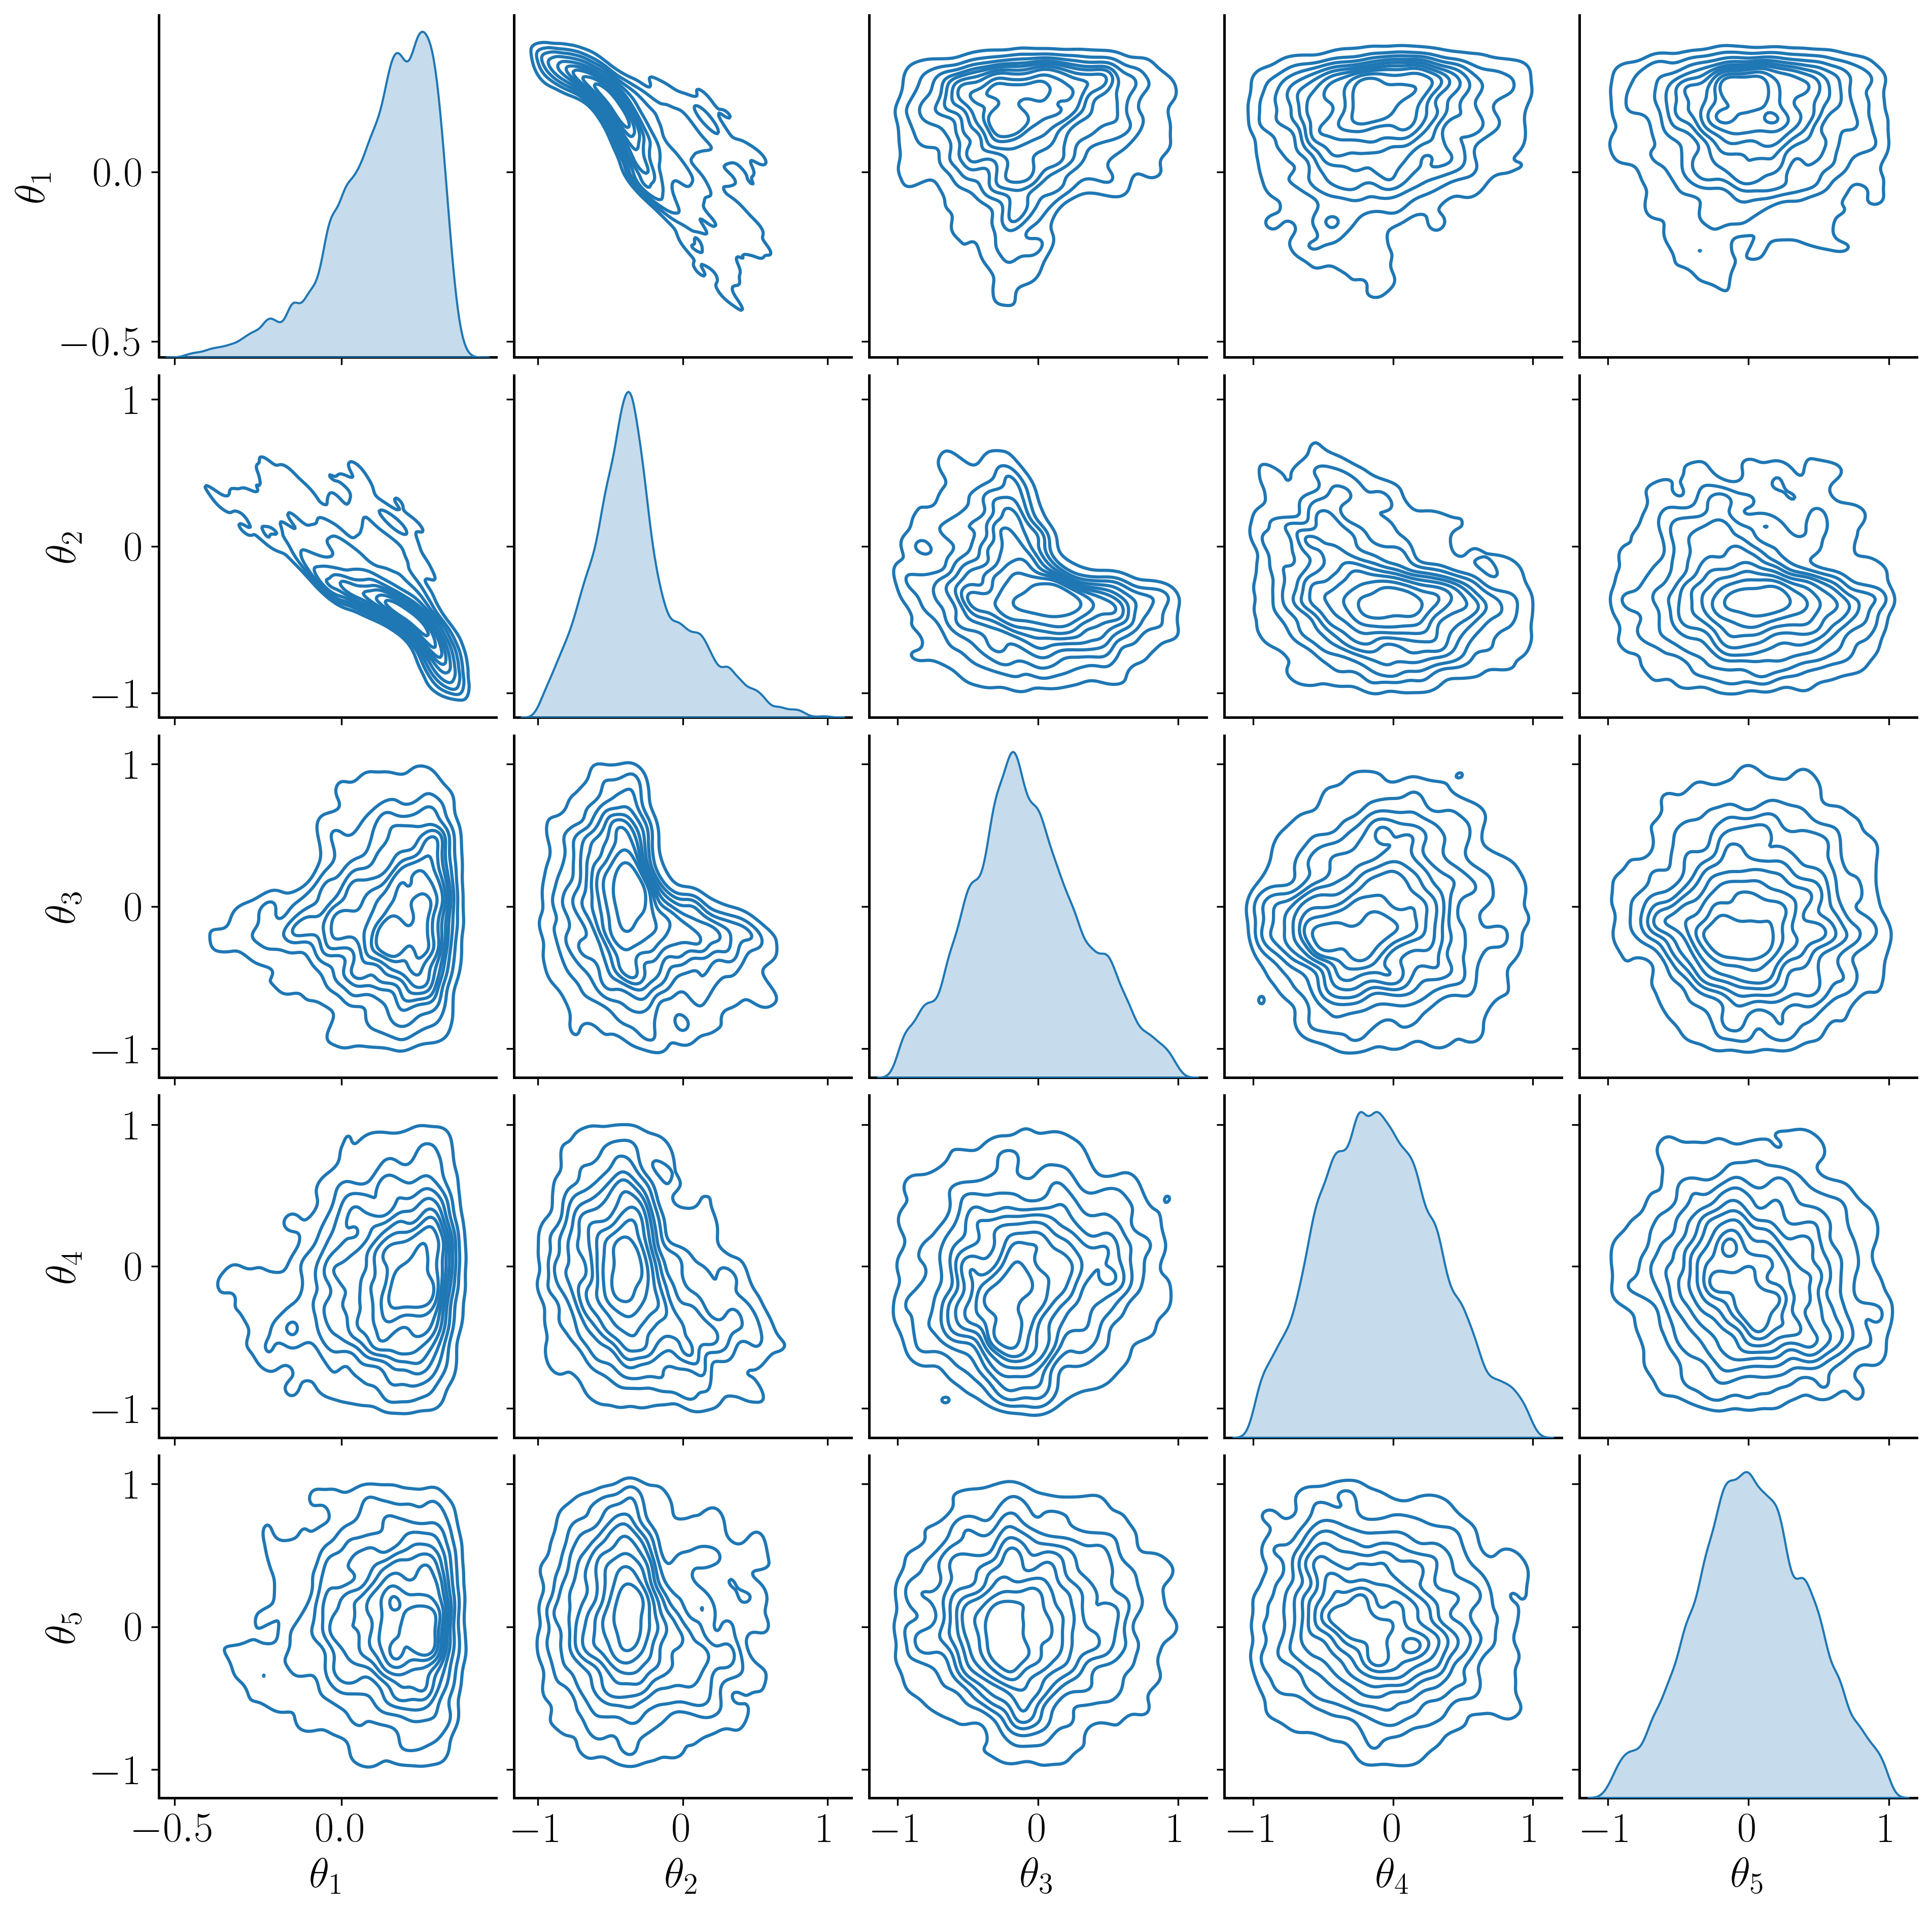
\includegraphics[width=1.0\linewidth]{Figures/kde_model4_DEsnooker.png}
\caption{Pairs plots (with a kernel density style) for all calibrated parameters of Model 4. The presented data is from 5 ensembles (last 1000 steps of each chain), run with DE-SNK, a wide prior and 1 observation for evaluating the likelihood. The parameters as presented here are untransformed (used for MCMC).}\label{fig_kde_model4_DEsnooker}
\end{figure}